\documentclass[a4paper,fleqn]{cas-sc}

\usepackage[authoryear,longnamesfirst]{natbib}

\usepackage[utf8]{inputenc}
\usepackage[english]{babel}

\usepackage{amsfonts,amssymb,amsmath,amsthm}
\usepackage{mathtools}

\usepackage{multirow}
\usepackage[shortlabels]{enumitem}

\usepackage{setspace}
\doublespacing

\usepackage{lineno}
\linenumbers

\usepackage{float}
\usepackage[section]{placeins}

\renewcommand{\topfraction}{0.9}
\renewcommand{\bottomfraction}{0.9}
\renewcommand{\textfraction}{0.05}
\renewcommand{\floatpagefraction}{0.7}

\numberwithin{equation}{section}

\graphicspath{{figs/}}

\def\tsc#1{\csdef{#1}{\textsc{\lowercase{#1}}\xspace}}
\tsc{LGCP}
\tsc{CNN}
\tsc{KDE}

\begin{document}
\let\WriteBookmarks\relax

\shorttitle{CNN with intensity features for LGCP}
\shortauthors{J. Romero et~al.}

\title[mode=title]{Parameter estimation in log-Gaussian Cox processes
via neural networks with spatial intensity features:
application to seismic events in Colombia}

\author[1]{Jason Romero}[orcid=0000-0000-0000-0000]
\cormark[1]
\ead{jamromeror@udistrital.edu.co}
\credit{Conceptualization, Methodology, Software, Writing - original draft}

\affiliation[1]{organization={Universidad Distrital Francisco Jos\'e de Caldas,
                Master's programme in Information and Communication Sciences},
                city={Bogot\'a},
                country={Colombia}}

\author[2]{Carlos Melo}
\credit{Supervision, Writing - review and editing}

\affiliation[2]{organization={Universidad Distrital Francisco Jos\'e de Caldas,
                Faculty of Engineering},
                city={Bogot\'a},
                country={Colombia}}

\author[3]{Oscar Melo}
\credit{Supervision, Writing - review and editing, Methodology}

\affiliation[3]{organization={Universidad Nacional de Colombia,
                Faculty of Sciences, Department of Statistics},
                city={Bogot\'a},
                country={Colombia}}

\cortext[1]{Corresponding author}

\begin{abstract}
The likelihood of a log-Gaussian Cox process (LGCP) has no closed form,
since its evaluation requires marginalising over a latent Gaussian field.
A recent line of work replaces the likelihood with a convolutional neural
network (CNN) trained on simulations, which predicts the parameters from
$\hat{L}(r)-r$ and the point count~$N$. So far this proposal had only
been tested on square windows, and the variance $\sigma^2$ and the
spatial range $s$ remain difficult to identify in practice. This work
adds eight scalar descriptors of the smoothed intensity field to the
CNN: variance, dispersion index and range ratio computed on quadrat
counts, together with variance, skewness, kurtosis, Shannon entropy and
coefficient of variation of the kernel density estimator. The method is
tested in a simulation study over the continental geometry of Colombia
and applied to the Colombian seismic catalogue for 2020. The descriptors
raise the $R^2$ for~$s$ from 0.57 to 0.83 ($+46.1$\,\%) and that of
$\sigma^2$ from 0.65 to 0.76 ($+17.3$\,\%); for $\mu$ a moderate
improvement is also observed (0.81 to 0.88, $+8.7$\,\%).
\end{abstract}

\begin{highlights}
\item We extend the Vihrs (2022) CNN with eight spatial intensity descriptors.
\item The descriptors provide first-order information absent in $\hat{L}(r)-r$.
\item LGCP: $R^2$ for the range $s$ rises from 0.57 to 0.83 and that of $\sigma^2$ from 0.65 to 0.76.
\item Tested by simulation over Colombia and applied to its seismic catalogue for 2020.
\end{highlights}

\begin{keywords}
Convolutional neural network \sep Log-Gaussian Cox process \sep
Spatial intensity features \sep Spatial point processes \sep
Seismicity \sep Simulation-based inference
\end{keywords}

\maketitle

\section{Introduction}
\label{sec:intro}

Many natural phenomena can be viewed as collections of random locations
in the plane: positions of trees in a forest, of nests in a reserve or
of seismic epicentres over a territory. The natural statistical object
to describe them is the spatial point process. Given an observed
pattern $\mathbf{x}=\{x_1,\ldots,x_n\}\subset W$ on a bounded window
$W\subset\mathbb{R}^2$, the goal is to recover the parameters
$\boldsymbol{\theta}$ of the model that generated it. The practical
obstacle is well known: in almost every model of interest the
likelihood involves intractable normalising constants or integrals over
latent variables, so direct maximum likelihood is not an option
\citep{MollerWaagepetersen2004}.

Within this family, the log-Gaussian Cox process (LGCP) is one of the
reference models for describing spatial aggregation \citep{Moller1998}.
Its intensity is a random surface $\Lambda(u)=\exp(Y(u))$, where $Y$ is
a Gaussian field with mean $\mu$ and covariance determined by the
variance $\sigma^2$ and the spatial range $s$. Evaluating
$p(\mathbf{x}\mid\boldsymbol{\theta})$ requires integrating over all
realisations of $Y$, a calculation with no closed-form solution. The
two classical routes are minimum contrast \citep{mincon83, mincon84},
which fits a theoretical summary statistic to its empirical estimate,
and composite likelihood \citep{complik}, which replaces the joint
likelihood with a product of pairwise contributions. Both yield point
estimates and rest on sensitive assumptions, such as the fitting range
or pairwise independence.

A different route is Bayesian inference via INLA-SPDE
\citep{Rue2009,toolboxINLA}, which represents the latent field as a
Gaussian Markov random field and approximates the posterior by nested
Laplace approximations. Unlike the previous methods, INLA-SPDE returns
full posteriors over $(\mu,\sigma^2,s)$, but its performance depends
strongly on the prior placed on the hyperparameters of the field.
Penalised complexity priors (PC priors) \citep{simpson2017penalising,
fuglstad2019constructing} are the current standard, and their
calibration relies on critical values typically set by expert
judgement. This dependence is an additional motivation for this work:
as developed in Section~\ref{sec:priors}, the estimates returned by the
CNN can serve as references for setting those values directly from the
observed pattern.

A more recent alternative is to treat estimation as a prediction
problem: many patterns are simulated with known parameters and a model
is trained to learn the inverse $\mathbf{x}\mapsto\boldsymbol{\theta}$.
This is the central idea of \emph{simulation-based inference}
\citep{Cranmer2020}. In spatial statistics, \citet{VIHRS2022} realised
it with a one-dimensional CNN that simultaneously estimates the
parameters of several point process models. The network takes
$\hat{L}(r)-r$ together with the point count $N$ as input and returns
$\hat{\boldsymbol{\theta}}$. Since it depends only on the ability to
simulate from the model, the strategy extends to any point process for
which a simulation procedure exists.

Two limitations of \citet{VIHRS2022} motivate the present extension.
The first is domain-related: the evaluation was carried out only on
unit square windows, while in real applications $W$ is usually an
irregular geographical region. That irregularity enters $\hat{L}(r)-r$
through the edge-correction weights and alters the shape of the curve
the network must interpret. The second is informational:
$D(r)=\hat{L}(r)-r$ is the only functional summary the network receives
and, as a second-order statistic, it describes pair structure but not
the spatial heterogeneity of the intensity. In an LGCP the surface
$\lambda(u)=\exp(Y(u))$ varies locally with an amplitude governed by
$\sigma^2$ and a scale given by $s$; both properties are averaged out
in $D(r)$. The practical consequence is that $\sigma^2$ and $s$ are
the hardest parameters to recover.

The guiding hypothesis of this work is that adding a few first-order
descriptors of the pattern to the CNN, complementary to $D(r)$,
improves the recovery of $\sigma^2$ and $s$ when the window is
irregular. The contributions of the article are:
\begin{enumerate}[(i)]
    \item a vector $\mathbf{f}\in\mathbb{R}^{8}$ of intensity
    descriptors built from quadrat counts and a kernel density
    estimator (\textit{kernel density estimation}), with an explicit
    relationship to the LGCP parameters;

    \item an extension of the architecture of \citet{VIHRS2022} that
    processes $\mathbf{f}$ through a sub-network before concatenating
    it with the dense layers;

    \item a simulation study over the continental contour of Colombia,
    an irregular domain with non-trivial edge effects, in which the
    proposed CNN is compared against the version without descriptors;

    \item the application to the Colombian seismic catalogue for 2020
    and a discussion of how to use the estimates to calibrate
    informative priors.
\end{enumerate}

The remainder of the article is organised as follows.
Section~\ref{sec:marco} reviews LGCPs, functional summary statistics
and one-dimensional CNNs. Section~\ref{sec:metodo} details the
methodology. Section~\ref{sec:simulacion} presents the simulation study
and Section~\ref{sec:aplicacion} the seismic application.
Section~\ref{sec:discusion} discusses results and future work.

The computations were performed in \texttt{R}~4.5.3 \citep{R}, with
\texttt{spatstat} \citep{spatstat} for the point processes and
\texttt{keras} \citep{keras_book,keras} for the networks. The scripts
are available in the ancillary files.

\section{Theoretical framework}
\label{sec:marco}

\subsection{Spatial point processes}
\label{sec:pp_theory}

A spatial point process $X$ on $\mathbb{R}^d$ is a random variable
whose values are locally finite subsets of $\mathbb{R}^d$
\citep{DaleyVereJones2008}. A realisation
$\mathbf{x}=\{x_1,\ldots,x_n\}$ is observed inside a bounded window
$W\subset\mathbb{R}^d$. The distribution of $X$ is characterised by its
product densities; in particular, the \emph{intensity function}
$\lambda\colon\mathbb{R}^d\to[0,\infty)$ is defined as the function
that satisfies
\begin{equation}
    \mathrm{E}\!\left[\sum_{x\in X\cap B}\!1\right]
    = \int_B \lambda(u)\,\mathrm{d}u
    \label{eq:intensity_def}
\end{equation}
for every bounded Borel set $B\subseteq\mathbb{R}^d$
\citep{MollerWaagepetersen2004}. If $\lambda(u)=\rho$ is constant for
all $u\in\mathbb{R}^d$, the process is called \emph{homogeneous} (or
first-order stationary). Otherwise, the process is said to be
\emph{non-homogeneous} or \emph{inhomogeneous}.

The simplest model is the \emph{homogeneous Poisson process} with
constant intensity $\rho$, in which the points are distributed
independently of one another. This model is the reference for
\emph{complete spatial randomness} (CSR). Most natural phenomena
deviate from CSR by exhibiting \emph{clustering} (points tend to
concentrate in certain regions) or \emph{regularity} (points tend to
repel each other) \citep{Diggle2014, spatstat}.

\subsubsection{Cox processes}

Cox processes generalise the Poisson process by allowing the intensity
to be itself random \citep{Cox1955}. Formally, a Cox process is defined
through a non-negative random field
$\Lambda=\{\Lambda(u)\}_{u\in\mathbb{R}^d}$, called the \emph{random
intensity}, such that, conditional on a realisation $\lambda(\cdot)$
of $\Lambda$, the process $X$ is an inhomogeneous Poisson process with
intensity function $\lambda(\cdot)$. The marginal (unconditional)
distribution of $X$ is obtained by marginalising over $\Lambda$:
\begin{equation}
    p(\mathbf{x}) = \mathrm{E}_{\Lambda}\!\left[
    \exp\!\left(-\int_W\!\Lambda(u)\,\mathrm{d}u\right)
    \prod_{i=1}^{n}\Lambda(x_i)\right].
    \label{eq:cox_likelihood}
\end{equation}

This marginalisation is in general analytically intractable, which is
the central difficulty for inference in Cox models
\citep{MollerWaagepetersen2004}.

\subsection{Log-Gaussian Cox processes}
\label{sec:lgcp_theory}

A particularly important case of Cox process arises when the logarithm
of the random intensity is a Gaussian field. A \emph{log-Gaussian Cox
process} (LGCP) \citep{Moller1998} is a Cox process whose random
intensity has the form
\begin{equation}
    \Lambda(u) = \exp(Y(u)), \quad u\in\mathbb{R}^d,
    \label{eq:lgcp_intensity}
\end{equation}
where $Y=\{Y(u)\}_{u\in\mathbb{R}^d}$ is a Gaussian random field with
mean function $\mathrm{E}[Y(u)]=m(u)$ and covariance function
$\mathrm{Cov}(Y(u),Y(v))=c(u,v)$.

The flexibility of the LGCP lies in the fact that the clustering
structure of the point pattern is governed by the properties of the
underlying Gaussian field: the mean function controls the global level
of intensity, while the covariance function determines the degree and
the scale of spatial clustering.

\subsubsection{Parameterisation used}

In this work the stationary parameterisation is adopted: $m(u)=\mu$
for a constant $\mu\in\mathbb{R}$ and a stationary and isotropic
covariance function from the Mat\'ern family
\citep{Matern1960, Stein1999}:
\begin{equation}
    c(u,v) = \sigma^2\,\mathcal{M}_{\nu}\!\left(\frac{\|u-v\|}{s}\right),
    \label{eq:cov_matern}
\end{equation}
where $\sigma^2>0$ is the marginal variance of the field, $s>0$ is the
scale parameter (spatial range), $\nu>0$ is the smoothness parameter,
and $\mathcal{M}_{\nu}$ denotes the Mat\'ern correlation function:
\begin{equation}
    \mathcal{M}_{\nu}(h) =
    \frac{2^{1-\nu}}{\Gamma(\nu)}\left(\sqrt{2\nu}\,h\right)^{\nu}
    K_{\nu}\!\left(\sqrt{2\nu}\,h\right),
    \label{eq:matern_corr}
\end{equation}
where $h=\|u-v\|/s$ is the Euclidean distance between the two points
$u,v\in\mathbb{R}^d$ being compared, normalised by the scale parameter
$s$, and $K_{\nu}$ is the modified Bessel function of the second kind.
Since the covariance depends only on the distance $\|u-v\|$ between the
two locations, and not on their absolute positions, the field $Y$ is
stationary and isotropic: the correlation between $Y(u)$ and $Y(v)$
decays with $h$ and is the same for any pair of points separated by
the same distance, regardless of direction or location within the
window.

\subsubsection{Properties of the stationary LGCP}

Under the previous parameterisation, the LGCP is a marginally
stationary process: the marginal intensity function (averaged over the
realisations of $Y$) is constant \citep{Moller1998}:
\begin{equation}
    \rho = \mathrm{E}[\Lambda(u)] = \exp(\mu + \sigma^2/2),
    \label{eq:lgcp_rho}
\end{equation}
and the expected number of points in the window is
$\mathrm{E}[N] = |W|\,\rho$. It is important to distinguish between the
\emph{marginal stationarity} of the process, which justifies the use
of summary statistics such as the $K$ function, and the
\emph{conditional inhomogeneity}: given a particular realisation of
the field $Y$, the intensity $\Lambda(u)=\exp(Y(u))$ varies spatially.

Note that if $\sigma^2=0$, the field $Y(u)=\mu$ is constant, the LGCP
reduces to a homogeneous Poisson process with intensity
$\rho=\exp(\mu)$, and the parameter $s$ becomes irrelevant.

\subsubsection{Intractability of the likelihood}

The likelihood of the LGCP requires evaluating the expectation in
\eqref{eq:cox_likelihood} over all realisations of the Gaussian field,
which involves an infinite-dimensional integral:
\begin{equation}
    p(\mathbf{x}\mid\boldsymbol{\theta}) =
    \mathrm{E}_{Y}\!\left[\exp\!\left(-\int_W\!e^{Y(u)}\,\mathrm{d}u\right)
    \prod_{i=1}^{n}e^{Y(x_i)}\right].
    \label{eq:lgcp_lik}
\end{equation}

No analytical solution exists for this integral. Existing inference
methods include: Laplace approximations via INLA
\citep{Rue2009,toolboxINLA}, which approximate the posterior using
Gaussian Markov random fields; minimum contrast
\citep{mincon83, mincon84}, which fits a theoretical summary statistic
to its empirical estimate; approximate Bayesian computation (ABC)
\citep{ABCoverview}; and methods based on composite likelihood
\citep{complik}. Each one introduces additional assumptions or
approximations. In this work an alternative approach based on
simulation and supervised learning is adopted
(Section~\ref{sec:cnn_theory}).

\subsubsection{Theoretical $K$ function of the LGCP}

For a stationary LGCP, the $K$ function admits an explicit expression
in terms of the covariance function of the Gaussian field
\citep{Moller1998}:
\begin{equation}
    K(r) = \pi r^2 + 2\pi\int_0^r\!\bigl(\exp(c(t))-1\bigr)\,t\,\mathrm{d}t,
    \label{eq:K_LGCP}
\end{equation}
where the first term corresponds to the $K$ function of the Poisson
process and the second quantifies the excess clustering induced by the
latent field. Since $\exp(c(t))-1\geq 0$ for every valid covariance
function, one has $K(r)\geq\pi r^2$ for all $r$, which implies
$L(r)\geq r$; that is, the LGCP is always a clustered process. The
functional form of $K(r)-\pi r^2$ depends jointly on $\sigma^2$
(which controls the amplitude of the integrand) and on $s$ (which
controls the scale at which $c(t)$ decays to zero).

\subsection{Functional summary statistics}
\label{sec:sumstats}

Functional summary statistics provide non-parametric descriptions of
the spatial dependence structure of a point process. The functions
relevant to this work are presented below.

\subsubsection{Ripley's $K$ function and $L$ function}

For a stationary point process with intensity $\rho$, \emph{Ripley's
$K$ function} \citep{Ripley76, Ripley88} is defined as the function
$K\colon[0,\infty)\to[0,\infty)$ such that $\rho K(r)$ is the expected
number of additional points of the process inside a disc of radius
$r$ centred at a typical point of the process:
\begin{equation}
    \rho\,K(r) = \mathrm{E}^{!o}\!\left[\sum_{x\in X\cap b(o,r)}1\right]
    \label{eq:K_def}
\end{equation}
where $\mathrm{E}^{!o}$ denotes the expectation under the reduced Palm
measure at the origin \citep{MollerWaagepetersen2004}. For a stationary
Poisson process in $\mathbb{R}^2$, $K(r)=\pi r^2$.

The \emph{$L$ function} is the variance-stabilising transformation
\citep{Besag1977}:
\begin{equation}
    L(r) = \sqrt{K(r)/\pi},
    \label{eq:L_function}
\end{equation}
so that $L(r)=r$ under CSR. The \emph{centred $L$ function}
\begin{equation}
    D(r) = L(r) - r
    \label{eq:D_function_theory}
\end{equation}
takes the value zero under CSR, positive values when there is
clustering ($K(r)>\pi r^2$) and negative values when there is
regularity ($K(r)<\pi r^2$). For the LGCP, \eqref{eq:K_LGCP} implies
that $D(r)\geq 0$ for all $r$.

\subsubsection{Estimation of $K$ and $L$ from data}

Given an observed point pattern $\mathbf{x}=\{x_1,\ldots,x_n\}\subset W$,
the non-parametric estimators of $K$ and $L$ are
\citep{Ripley88, spatstat}:
\begin{align}
    \widehat{K}_{\mathbf{x}}(r) &= \frac{|W|}{n(n-1)}\sum_{i=1}^{n}
    \sum_{\substack{j=1\\j\neq i}}^{n}
    \mathbf{1}[\|x_i-x_j\|\leq r]\,e_{ij}(r),
    \label{eq:K_hat} \\
    \widehat{L}_{\mathbf{x}}(r) &= \sqrt{\widehat{K}_{\mathbf{x}}(r)/\pi},
    \label{eq:L_hat}
\end{align}
where $|W|$ is the area of the window and $e_{ij}(r)$ are
edge-correction weights that compensate for points not observed
outside $W$.

\subsubsection{Edge correction for irregular windows}

The choice of edge correction is especially relevant when the window
$W$ has irregular geometry. In this work the \emph{border correction}
is used, in which only the points $x_i$ whose distance to the boundary
of $W$ is at least $r$ are considered:
\begin{equation}
    \widehat{K}_{\mathrm{bord}}(r) = \frac{|W|}{n_r(n_r-1)}
    \sum_{\substack{i:\,d(x_i,\partial W)\geq r}}
    \sum_{\substack{j\neq i}}
    \mathbf{1}[\|x_i-x_j\|\leq r],
    \label{eq:K_border}
\end{equation}
where $n_r = \#\{i : d(x_i,\partial W)\geq r\}$ and $d(x_i,\partial W)$
is the distance from $x_i$ to the boundary of $W$ \citep{spatstat}.
This correction is appropriate for non-convex windows because it does
not require computing the proportion of a circle contained within $W$
(as Ripley's isotropic correction does), which can be geometrically
complex for irregular boundaries.

The estimated $D(r)$ function is defined as
\begin{equation}
    \hat{D}(r) = \widehat{L}(r) - r = \sqrt{\widehat{K}(r)/\pi} - r.
    \label{eq:D_function}
\end{equation}

\subsubsection{Other functional statistics}

Other important functional statistics include the nearest-neighbour
distance distribution function $G(r)$, the empty-space function
$F(r)$, and the function $J(r)=(1-G(r))/(1-F(r))$
\citep{VanLieshoutBaddeley1996, MollerWaagepetersen2004}. Although
these functions provide complementary information, in this work $D(r)$
is used exclusively as the summary statistic, following the choice of
\citet{VIHRS2022}, since the $K$ function has a direct analytical
relationship with the LGCP parameters via \eqref{eq:K_LGCP}.

\subsection{Simulation-based inference with neural networks}
\label{sec:cnn_theory}

\emph{Simulation-based inference} (SBI) groups a set of methods that
dispense with the explicit evaluation of the likelihood, replacing it
with the ability to simulate from the generative model
\citep{Cranmer2020}. The general approach consists of: (i) generating a
training set
$\{(\boldsymbol{\theta}^{(i)},\mathbf{x}^{(i)})\}_{i=1}^{n}$ with
$\boldsymbol{\theta}^{(i)}\sim p(\boldsymbol{\theta})$ and
$\mathbf{x}^{(i)}\sim p(\mathbf{x}\mid\boldsymbol{\theta}^{(i)})$;
(ii) training a statistical or machine-learning model that learns the
relationship $\mathbf{x}\mapsto\boldsymbol{\theta}$; and (iii) applying
the trained model to the observed data to obtain
$\hat{\boldsymbol{\theta}}$.

In the context of spatial point processes, \citet{VIHRS2022} proposed
using a one-dimensional CNN as the prediction model, motivated by the
nature of the vector
$\mathbf{L}=(\hat{L}(r_1)-r_1,\ldots,\hat{L}(r_T)-r_T)^\top$, whose
values are indexed by the distance $r\in[0,r_{\max}]$ and which has
sequential behaviour with local dependence. The $L(r)$ function shows
different structure for $r < s$, $r \approx s$ and $r > s$; this
structure is \emph{local in $r$} and is exactly the type of pattern
that convolutional filters are designed to detect. Finally, the
function $r\mapsto\hat{L}(r)$ is smooth (as a function of $r$), which
means that neighbouring values are highly correlated
\citep{Kiranyaz2021}. The CNN takes as input the functional summary
statistic $D(r)=\hat{L}(r)-r$, which encodes the second-order
structure of the pattern, together with the point count $N$, and
produces the estimates $\hat{\boldsymbol{\theta}}$ as output. The
complete mathematical formulation of these operations is presented in
Section~\ref{sec:metodo}.

\section{Proposed methodology}
\label{sec:metodo}

The curve $D(r)=\hat{L}(r)-r$ describes the second-order structure of
the pattern but leaves out the spatial heterogeneity of the intensity.
In an LGCP, that heterogeneity is precisely the signal that carries
information about $\sigma^2$ (local amplitude of
$\lambda(u)=\exp(Y(u))$) and about $s$ (scale at which that variation
decorrelates). The proposal is to summarise that heterogeneity in a
scalar vector $\Phi\colon\mathbf{x}\mapsto\mathbf{f}\in\mathbb{R}^{8}$
and feed it to the CNN as an auxiliary input, without modifying the
branch that processes $D(r)$ in \citet{VIHRS2022}.

\subsection{Spatial intensity descriptors}
\label{sec:features}

Given an observed point pattern $\mathbf{x}=\{x_1,\ldots,x_n\}\subset W$,
eight scalar descriptors that capture the spatial heterogeneity of the
smoothed intensity field are extracted, grouped into two families
(see Figure~\ref{fig:simulation_pipeline}).

\begin{figure}[pos=H]
    \centering
    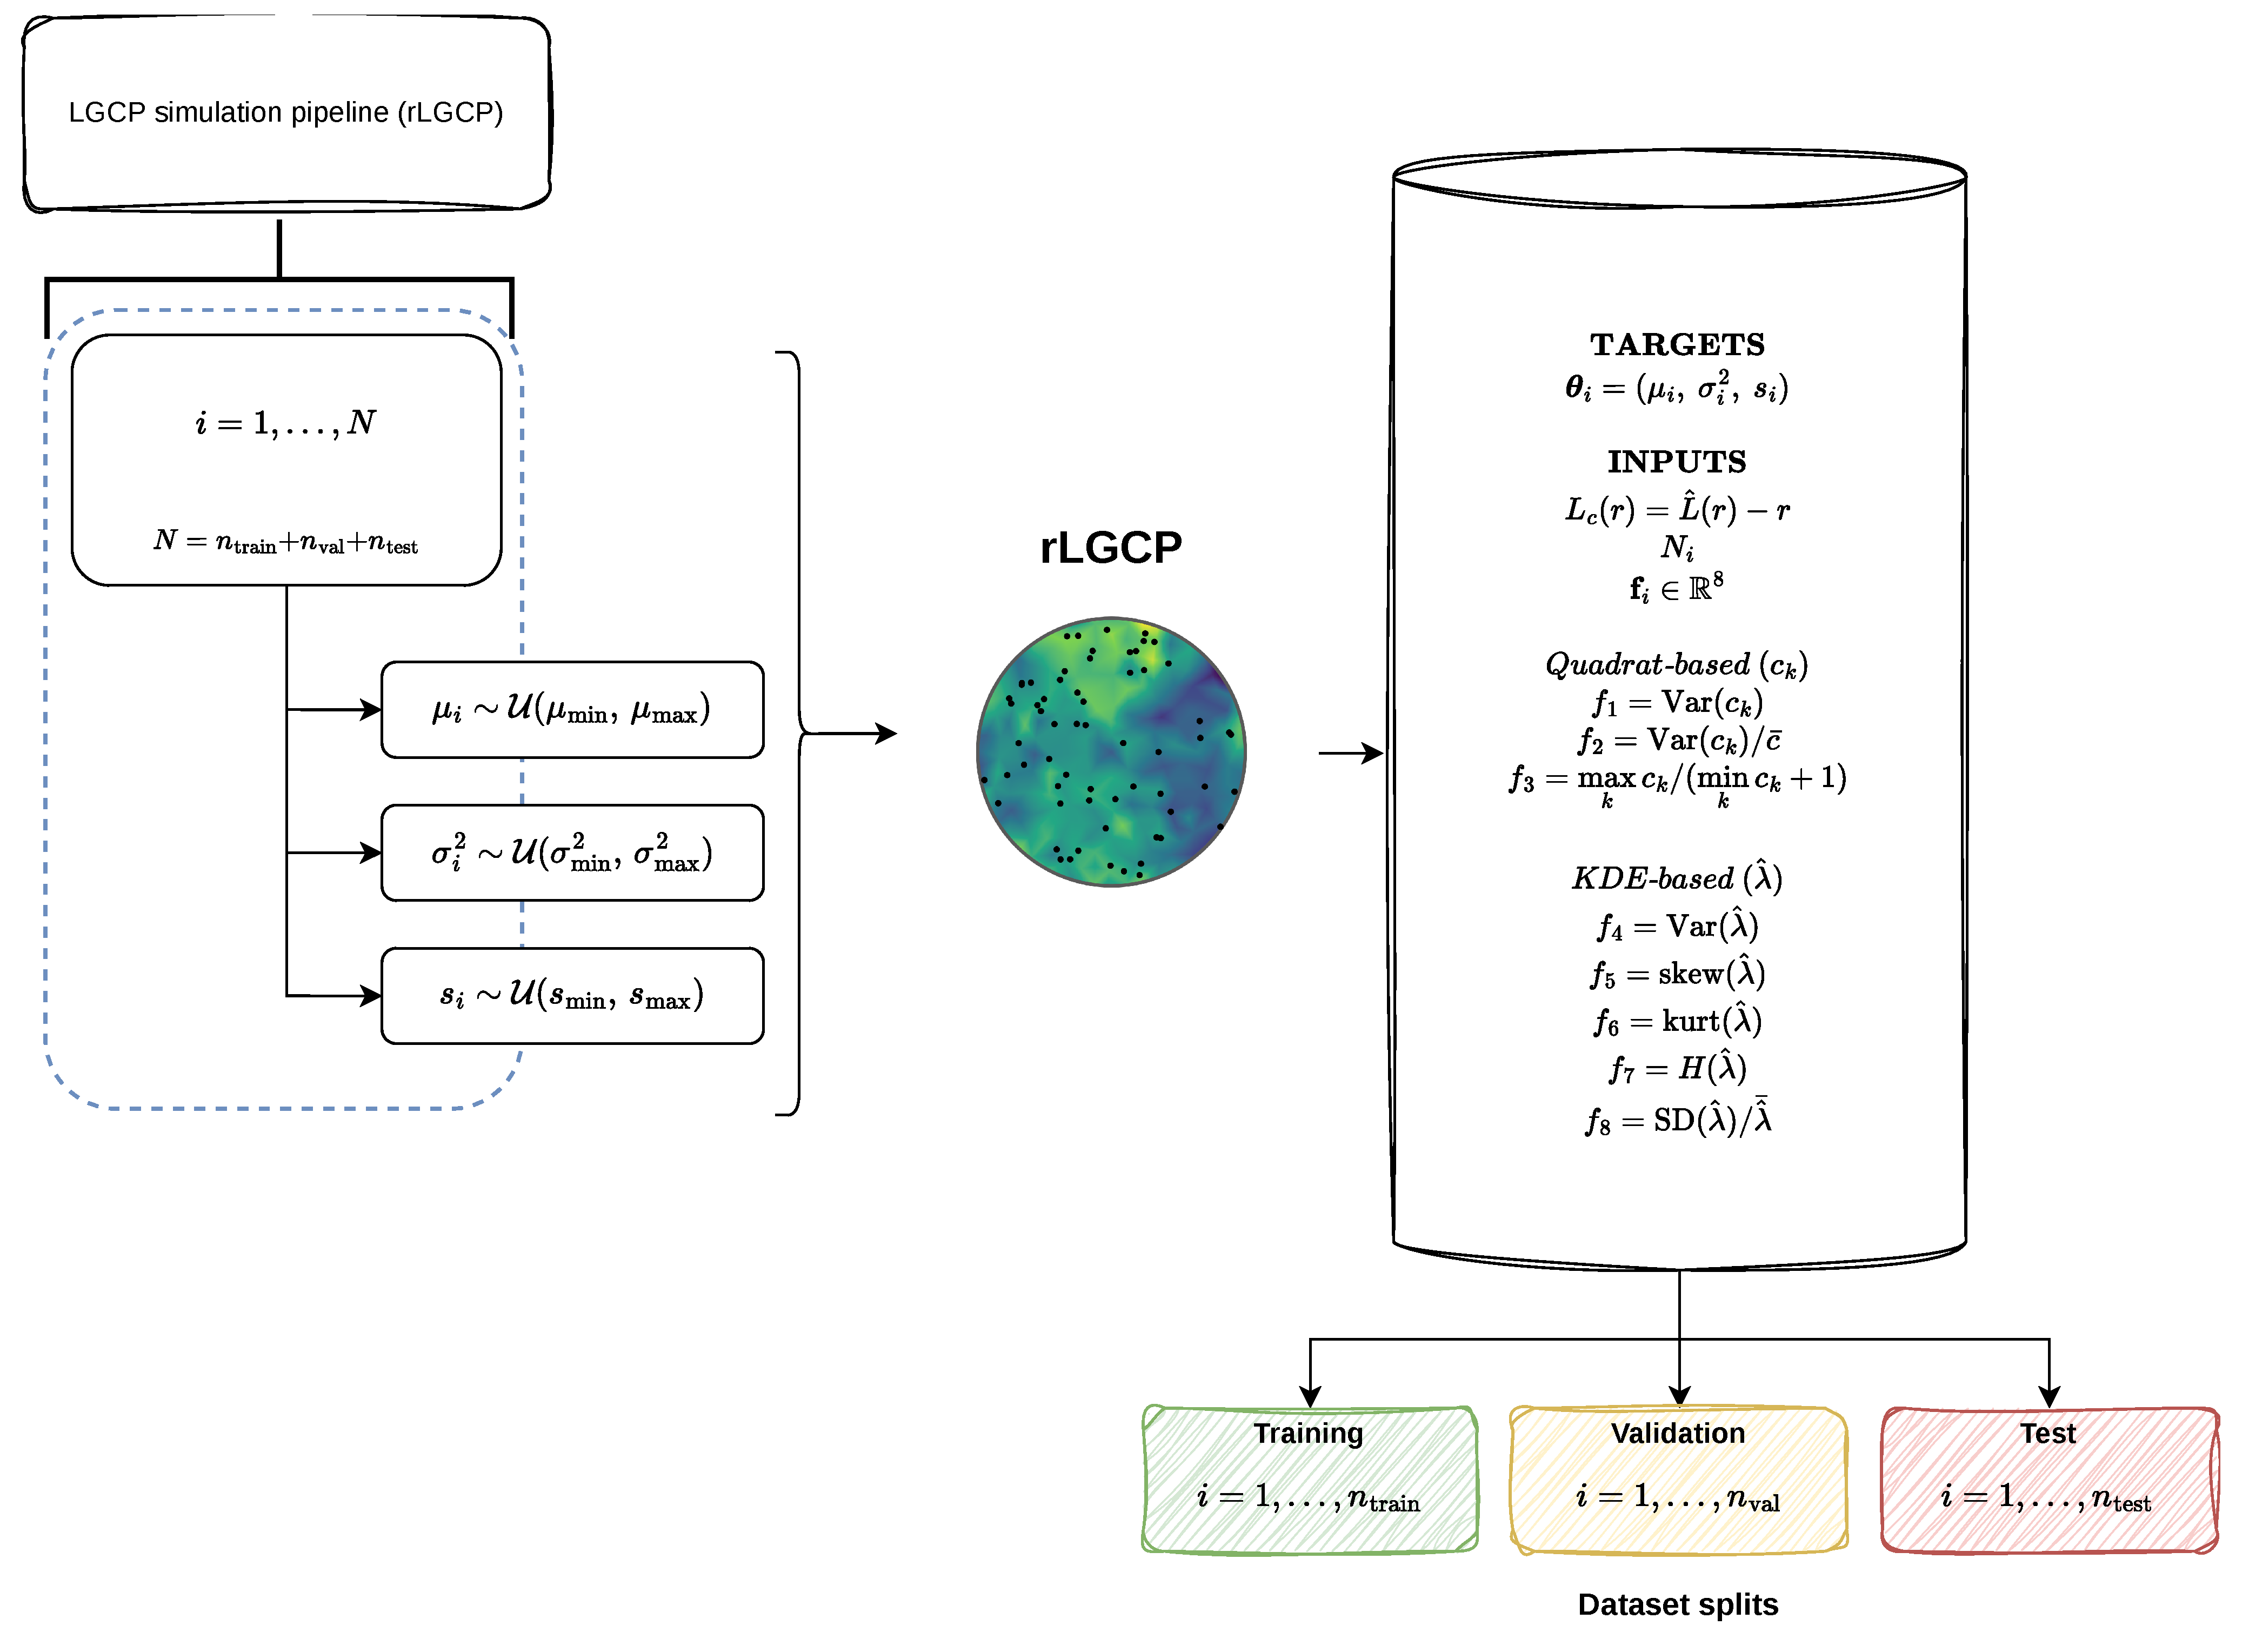
\includegraphics[width=0.75\linewidth]{diagrammethodology.pdf}
\caption{Simulation procedure for generating the training set:
for each realisation $i$, the LGCP parameters $(\mu_i, \sigma^2_i, s_i)$
are sampled from uniform distributions; a point pattern $\mathbf{x}_i$
is simulated via \texttt{rLGCP} (spatstat) on the window $W$ with
Mat\'ern covariance ($\nu=1$); the centred $L$ function
$D(r)=\hat{L}(r)-r$ is estimated with edge correction and the eight
intensity descriptors $\mathbf{f}_i = \Phi(\mathbf{x}_i) \in
\mathbb{R}^{8}$ are extracted via quadrat counts and kernel density
estimation. Each training example stores
$\boldsymbol{\theta}_i = (\mu_i,\sigma^2_i,s_i)$ as the label and
$(D(r),\, N_i,\, \mathbf{f}_i)$ as the input.}
\label{fig:simulation_pipeline}
\end{figure}


\subsubsection{Descriptors based on quadrat counts}

The window $W$ is divided into an $n_q\times n_q$ grid of quadrats
(with $n_q=5$) and the number of points $c_k$ in each quadrat
$k=1,\ldots,K$ intersecting $W$ is counted:

\begin{enumerate}[label=(\roman*),leftmargin=*,itemsep=0.6em]
\item \textbf{Variance of counts:}
\begin{equation}
f_1 = S_c^2 \coloneqq \frac{1}{K-1}\sum_{k=1}^{K}(c_k - \bar{c})^2.
\label{eq:f1_var_c}
\end{equation}
Under a homogeneous Poisson process, the quadrat counts have variance
equal to their mean, $\bar{c}$. In an LGCP, the latent field induces
overdispersion: some quadrats accumulate many points and others very
few, so that $S_c^2 > \bar{c}$. The excess grows with $\sigma^2$,
which controls the amplitude of the fluctuations of $\Lambda(u)$.

\item \textbf{Dispersion index:}
\begin{equation}
f_2 = \mathrm{VMR} \coloneqq \frac{S_c^2}{\bar{c}}.
\label{eq:f2_vmr}
\end{equation}
Variance-to-mean ratio (VMR) of the counts, a classical statistic to
quantify the departure from Poisson \citep{Diggle2014}. It equals 1
under homogeneous Poisson and exceeds 1 under clustering; its
magnitude depends jointly on $\sigma^2$ and $s$.

\item \textbf{Range ratio:}
\begin{equation}
f_3 = \frac{\max_k c_k}{\min_k c_k + 1}.
\label{eq:f3_range}
\end{equation}
Ratio between the maximum and the minimum count per quadrat (with a
$+1$ in the denominator to avoid division by zero). It is sensitive to
the presence of \emph{hotspots}: high values indicate that at least
one sub-region concentrates many more points than the rest, a
characteristic behaviour of large $\sigma^2$.
\end{enumerate}

\subsubsection{Descriptors based on kernel density estimation}

To capture the heterogeneity at a finer resolution than that of the
quadrats, the smoothed intensity field $\hat{\lambda}(u)$ is estimated
through a Gaussian kernel density estimator (KDE)
\citep{Silverman1986}, a standard technique in the analysis of point
patterns \citep{Illian2008, WiegandMoloney2013}, with fixed bandwidth
$h$, evaluated on a $64\times 64$ pixel grid:
\begin{equation}
    \hat{\lambda}(u) = \sum_{i=1}^{n} K_h(u - x_i), \quad
    K_h(u) = \frac{1}{2\pi h^2}\exp\!\left(-\frac{\|u\|^2}{2h^2}\right).
    \label{eq:kde}
\end{equation}

The bandwidth is fixed at $h=50\,000$\,m (50\,km), so that all
simulations are smoothed at the same scale and the resulting
descriptors are comparable across patterns with different $N$. Let
$\{\hat{\lambda}_j\}_{j=1}^{J}$ be the set of KDE values at the $J$
pixels falling inside $W$. From this set, five descriptors are
defined:
\begin{enumerate}[label=(\roman*),leftmargin=*,itemsep=0.6em]
\item \textbf{KDE variance:}
\begin{equation}
f_4 = S_{\hat{\lambda}}^2 \coloneqq
    \frac{1}{J-1}\sum_{j=1}^{J}(\hat{\lambda}_j - \bar{\hat{\lambda}})^2.
\label{eq:f4_var_kde}
\end{equation}
Summarises the spatial variability of the smoothed intensity field and
acts as a direct proxy for $\sigma^2$: since
$\mathrm{Var}[\Lambda(u)]=\exp(2\mu+\sigma^2)(\exp(\sigma^2)-1)$ is
increasing in $\sigma^2$, latent fields with greater variance produce
surfaces $\hat{\lambda}(u)$ that are more dispersed between pixels.

\item \textbf{KDE skewness:}
\begin{equation}
f_5 = \gamma_{\hat{\lambda}} \coloneqq
    \frac{J^{-1}\sum_{j=1}^{J}(\hat{\lambda}_j -
    \bar{\hat{\lambda}})^3}{(S_{\hat{\lambda}})^3}.
\label{eq:f5_skew}
\end{equation}
Third standardised moment of the intensity distribution. The
transformation $\Lambda(u)=\exp(Y(u))$ asymmetrically amplifies the
positive fluctuations of the Gaussian field, so that when $\sigma^2$
is large a few \emph{hotspots} appear with intensity well above the
typical value, which translates into high positive values of
$\gamma_{\hat{\lambda}}$.

\item \textbf{KDE kurtosis:}
\begin{equation}
f_6 = \kappa_{\hat{\lambda}} \coloneqq
    \frac{J^{-1}\sum_{j=1}^{J}(\hat{\lambda}_j -
    \bar{\hat{\lambda}})^4}{(S_{\hat{\lambda}}^2)^2} - 3.
\label{eq:f6_kurt}
\end{equation}
Excess kurtosis relative to the normal. With high $\sigma^2$, the
spatial distribution of $\hat{\lambda}(u)$ becomes leptokurtic, with
heavy tails and frequent extreme values; with low $\sigma^2$ it
flattens and the kurtosis approaches zero.

\item \textbf{Normalised Shannon entropy:}
\begin{equation}
f_7 = H_{\hat{\lambda}} \coloneqq
    -\frac{\sum_{j=1}^{J} p_j\log p_j}{\log J}, \quad
    p_j = \frac{\hat{\lambda}_j}{\sum_{l=1}^{J}\hat{\lambda}_l}.
\label{eq:f7_entropy}
\end{equation}
Quantifies the spatial uniformity of the intensity on a $[0,1]$ scale:
values close to 1 correspond to practically homogeneous fields, while
low values indicate concentration of intensity in a few regions. The
use of entropy as a spatial descriptor of seismicity had already been
explored by \citet{Despaigne2017}, who studied it as a precursor of
large earthquakes based on the distribution of hypocentres. This
descriptor is especially informative about $s$, since a small range
generates localised patches of high intensity (low entropy) and a
large range produces smoother surfaces (high entropy).

\item \textbf{Coefficient of variation:}
\begin{equation}
f_8 = \mathrm{CV}_{\hat{\lambda}} \coloneqq
    \frac{S_{\hat{\lambda}}}{\bar{\hat{\lambda}}}.
\label{eq:f8_cv}
\end{equation}
Ratio between the standard deviation and the mean of the field. By
normalising $f_4$ by the mean intensity level, its dependence on
$\mu$ is reduced, yielding a descriptor centred on the \emph{relative
heterogeneity} of the field.
\end{enumerate}

The eight descriptors are grouped into the feature-extraction operator
\begin{equation}
    \Phi(\mathbf{x}) = \mathbf{f} =
    (f_1,f_2,\ldots,f_{8})^{\top} \in \mathbb{R}^{8}.
    \label{eq:phi}
\end{equation}

\subsection{CNN architecture}
\label{sec:cnn_extended}

The main input of the network is the centred curve
$\mathbf{D}=(D(r_1),\ldots,D(r_m))^{\top}\in\mathbb{R}^{m}$, evaluated
at $m=128$ equally spaced values. This curve encodes the entire
spatial dependence structure of the point pattern: its shape,
amplitude and decay rate reflect the parameters $(\mu,\sigma^2,s)$ of
the underlying LGCP. The goal of the network is to learn to extract
this information automatically from the discrete signal $\mathbf{D}$.

\subsubsection{Convolutional processing of the $D(r)$ curve}

The standardised curve
$\tilde{\mathbf{D}}\in\mathbb{R}^{m\times 1}$ enters as a
one-dimensional signal with a single channel. It is processed through
a block of three 1D convolutional layers, each with $p=64$ filters of
size $q=7$. In each layer, the $p$ filters traverse the input
sequence via a sliding window of $q$ consecutive positions; at each
position $j$, the $i$-th filter computes
\begin{equation}
    S^{(\ell+1)}_{j,i} = \mathrm{relu}\!\left(
    b^{(\ell)}_i + \sum_{h=1}^{c_\ell}\sum_{l=0}^{q-1}
    W^{(\ell)}_{i,l+1,h}\; S^{(\ell)}_{j+l,\,h}
    \right)
    \label{eq:conv1d}
\end{equation}
where $\mathbf{W}^{(\ell)}_i\in\mathbb{R}^{q\times c_\ell}$ and
$b^{(\ell)}_i$ are the weights and the bias of the filter, and
$c_\ell$ is the number of channels of the preceding layer ($c_1=1$
for the first layer, $c_\ell=64$ for the following ones). The
activation function $\mathrm{relu}(x)=\max(0,x)$ introduces the
non-linearity necessary to capture complex relationships in the curve.

The kernel size $q=7$ allows each filter to simultaneously observe 7
consecutive values of $D(r)$, which corresponds to a representative
segment of the range of distances.

After each of the first two convolutional layers a \emph{max pooling}
operation with window $w=5$ is applied, which selects the maximum
value in contiguous blocks of 5 positions. This progressive reduction
of the sequence dimension has a twofold effect: it decreases the
number of parameters of the network and confers some invariance to
small shifts in the curve \citep{biscione2021cnns}.

After the third convolution, the resulting sequence is flattened into
a vector $\mathbf{z}_{\mathrm{conv}}\in\mathbb{R}^{d_c}$, which is a
compact and learned representation of the patterns that govern the
full $D(r)$ curve and is then fed into the learning process through
\emph{backpropagation}.

\subsubsection{Fusion with auxiliary inputs}

The vector $\mathbf{z}_{\mathrm{conv}}$ captures the information
contained in the \emph{shape} of the curve, but it does not directly
incorporate the information about the point count of the simulated
process, as defined by \citet{VIHRS2022}, nor the intensity
descriptors defined in Section~\ref{sec:features}. These two
complementary sources of information are incorporated at the
concatenation point: the vector
$\mathbf{z}_{\mathrm{conv}} \in \mathbb{R}^{d_z}$, obtained after
flattening, is extended with the scalar $\tilde{N} \in \mathbb{R}$
and the vector of global descriptors
$\tilde{\mathbf{f}} \in \mathbb{R}^{8}$, resulting in a single vector
of dimension $\mathbb{R}^{d_z + 9}$ that serves as input to the dense
layer block (see Figure~\ref{fig:NNet_extended}):
\begin{equation}
    \mathbf{a}^{(0)} = \bigl[\mathbf{z}_{\mathrm{conv}};\;\tilde{N};\;
    \tilde{\mathbf{f}}\bigr] \in \mathbb{R}^{d_c + 1 + 8}
    \label{eq:concat}
\end{equation}
where $\tilde{N}=(N-\mu_N)/\sigma_N$ is the standardised point count
and $\tilde{\mathbf{f}}\in\mathbb{R}^{8}$ is the standardised
intensity descriptor vector, with
$\tilde{f}_k=(f_k-\mu_{f_k})/\sigma_{f_k}$ for each component.

\subsubsection{Dense layers and output}

The concatenated vector passes through two dense layers with ReLU
activation, of 64 and 32 units respectively. The first layer
processes the combined information from the convolutional block and
the auxiliary descriptors, while the reduction to 32 units in the
second layer forces the network to retain only the most relevant
information for parameter estimation.

Finally, a linear layer without activation produces a vector of three
values $\hat{\boldsymbol{\theta}} = (\hat{\mu},\, \hat{\sigma}^2,\,
\hat{s})$, corresponding to the parameters of the model. The complete
architecture is illustrated in Figure~\ref{fig:NNet_extended}.

\begin{figure}[pos=H]
\centering
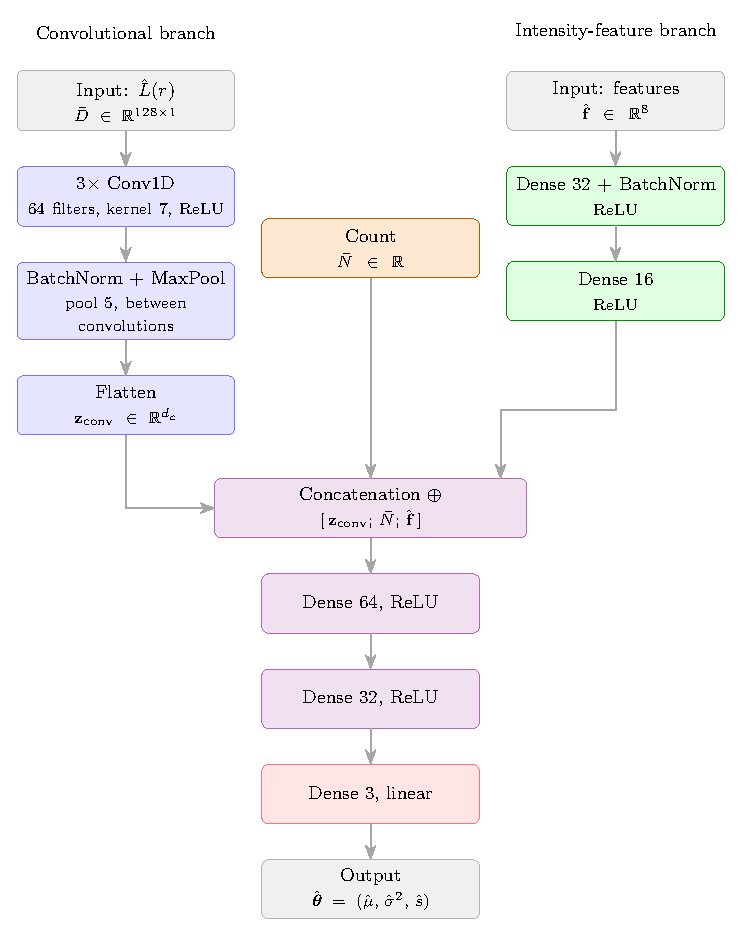
\includegraphics[width=0.45\linewidth]{cnn_architecture.pdf}
\caption{Proposed CNN architecture. At the concatenation point
($\oplus$), $\mathbf{z}_{\mathrm{conv}}$, the standardised count
$\tilde{N}$ and the 8 intensity descriptors $\tilde{\mathbf{f}}$ are
fused. Two dense layers with ReLU activation and a linear output
layer produce the estimate
$\hat{\boldsymbol{\theta}}=(\hat{\mu},\hat{\sigma}^2,\hat{s})$.}
\label{fig:NNet_extended}
\end{figure}

\subsection{Loss function and optimisation}
\label{sec:loss}

Let $\{(\tilde{\mathbf{D}}^{(i)}, \tilde{N}^{(i)},
\tilde{\mathbf{f}}^{(i)},
\tilde{\boldsymbol{\theta}}^{(i)})\}_{i=1}^{n_{\mathrm{train}}}$
denote the training set. Let
$g_{\boldsymbol{\omega}}(\tilde{\mathbf{D}}, \tilde{N},
\tilde{\mathbf{f}})$ denote the function implemented by the network
with trainable parameters $\boldsymbol{\omega}$. The loss function is
the mean squared error:
\begin{equation}
    \mathcal{L}(\boldsymbol{\omega}) = \frac{1}{n_{\mathrm{train}}}
    \sum_{i=1}^{n_{\mathrm{train}}}
    \bigl\|g_{\boldsymbol{\omega}}(\tilde{\mathbf{D}}^{(i)},
    \tilde{N}^{(i)}, \tilde{\mathbf{f}}^{(i)})
    - \tilde{\boldsymbol{\theta}}^{(i)}\bigr\|_2^2.
    \label{eq:loss}
\end{equation}
Minimisation is performed using the Adam optimiser \citep{adam}, with
mini-batches of size $B=64$.

The available data are split into three sets. The $n_{\mathrm{train}}$
simulations are devoted to training; of these, 80\,\% are effectively
used to update the network weights and the remaining 20\,\% constitute
the \emph{validation} set, used to monitor performance during
training. Additionally, a \emph{test} set with $n_{\mathrm{test}}$
simulations is generated independently, using the same parameter
ranges, which does not participate in any training stage or in model
selection, and is reserved exclusively for assessing the
generalisation capability of the trained network.

To prevent overfitting, \emph{early stopping} is used: training stops
when the validation loss does not improve over 15 consecutive epochs,
restoring the weights corresponding to the epoch of lowest observed
validation loss. Additionally, the \texttt{ReduceLROnPlateau}
\emph{callback} is employed, which halves the learning rate when the
validation loss does not improve for 7 epochs, with a minimum rate of
$10^{-6}$. The convolutional network includes \emph{batch
normalisation} after each convolutional layer to stabilise training.

\section{Simulation study}
\label{sec:simulacion}

In this section, the ability of the proposed method to recover the
parameters of an LGCP is evaluated through a simulation study. Unlike
the study of \citet{VIHRS2022}, which used a unit square window, here
the continental geometry of Colombia is used as the observation
window, which introduces the typical challenges of irregular domains.
Before defining the configuration of the study, an exploratory
analysis of the seismic catalogue is presented that motivates the
choice of parameter ranges.

\subsection{Exploratory analysis of the seismic pattern}
\label{sec:analisis_csr}

The catalogue of continental seismic events in Colombia for 2020 was
used, obtained from the Servicio Geol\'ogico Colombiano, with a total
of $14\,346$ events recorded across the continental territory,
projected to the EPSG:3116 reference system (planar coordinates in
metres). Figure~\ref{fig:mapa_sismos} shows the spatial distribution
of the $N$ events recorded over the observation window $W$,
corresponding to the simplified continental contour of Colombia with
$|W| \approx 1.14 \times 10^{12}$\,m$^2$.

\begin{figure}[pos=H]
\centering
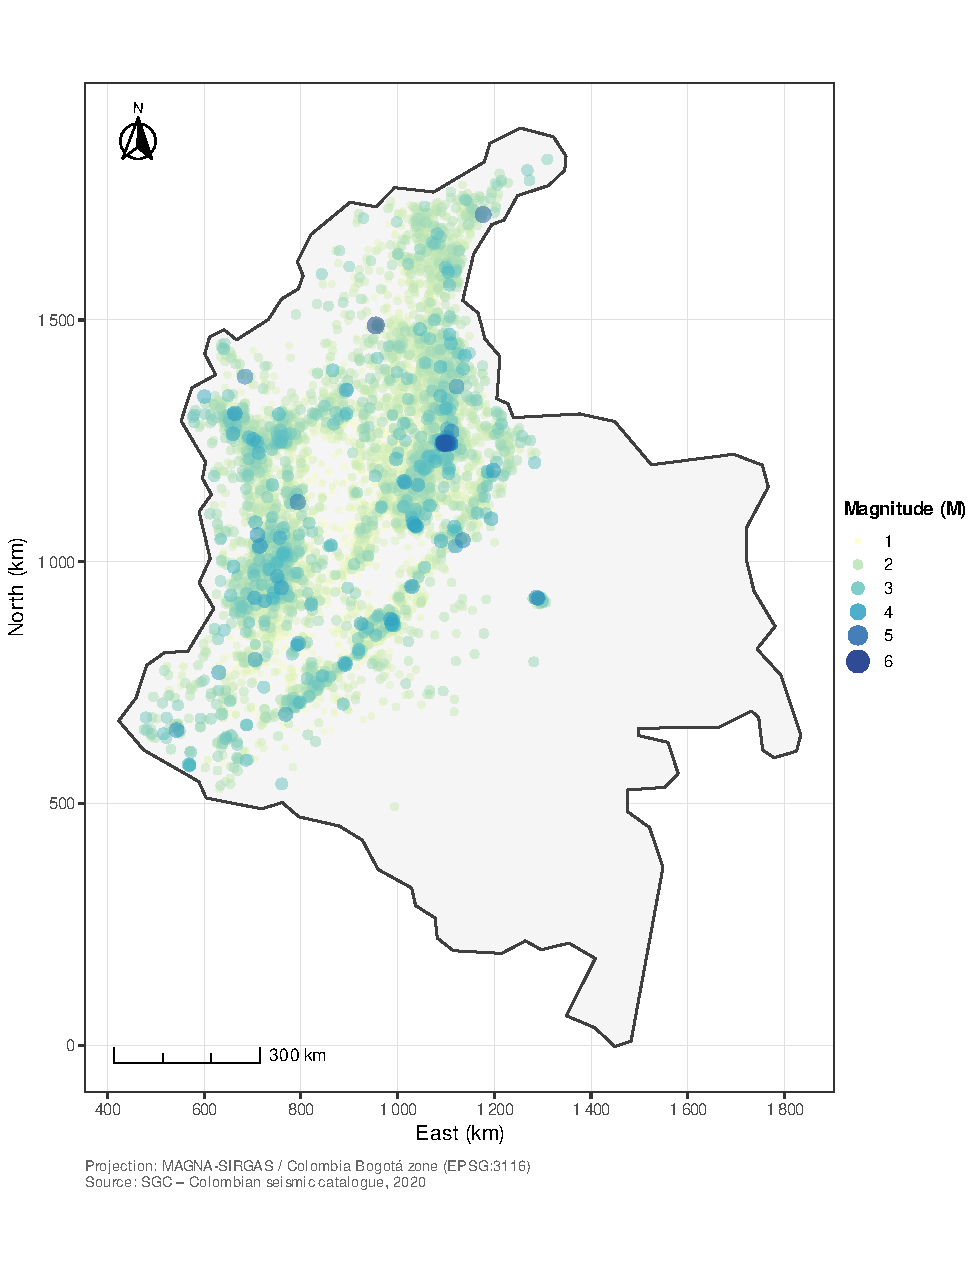
\includegraphics[width=0.45\linewidth]{earthquakes_map_2020.pdf}
\caption{Spatial distribution of the seismic events recorded in
continental Colombia during 2020.}
\label{fig:mapa_sismos}
\end{figure}

\subsubsection{Complete spatial randomness analysis}

The complete spatial randomness analysis was performed using the
Pearson $\chi^2$ test, based on a tessellation of the region of study
into quadrats resulting from dividing the window $W$ into 6 horizontal
strips and 6 vertical strips with respect to the $X$ and $Y$ axes,
respectively (Figure~\ref{fig:cuadrat_count}). Since the window is
irregular, the effective number of quadrats with positive area is 29.
Table~\ref{tab:csr} summarises the results of the test.

\begin{table}[pos=H]
\centering
\caption{Results of the $\chi^2$ test for complete spatial randomness
(quadrat test).}
\label{tab:csr}
\begin{tabular*}{\tblwidth}{@{} LCC @{}}
\toprule
\textbf{Statistic} & \textbf{Value} & \textbf{Interpretation} \\
\midrule
$\chi^2$ & $288.60$ &
    \multirow{2}{*}{\shortstack[l]{$p < 2.2\times 10^{-16}$\\Rejection of CSR}} \\
Degrees of freedom & 28 & \\
\midrule
Effective quadrats & 29 & Irregular window \\
\bottomrule
\end{tabular*}
\end{table}

The statistic $\chi^2 = 288.60$ with $p < 2.2\times 10^{-16}$ leads to
rejection of CSR at the 5\,\% level; the observed counts are far from
those a homogeneous Poisson process would produce. The result agrees
with that reported by \citet{TesisColegas} for the period 2005--2015
and rules out fitting a homogeneous Poisson process to Colombian
seismicity.

\begin{figure}[pos=H]
\centering
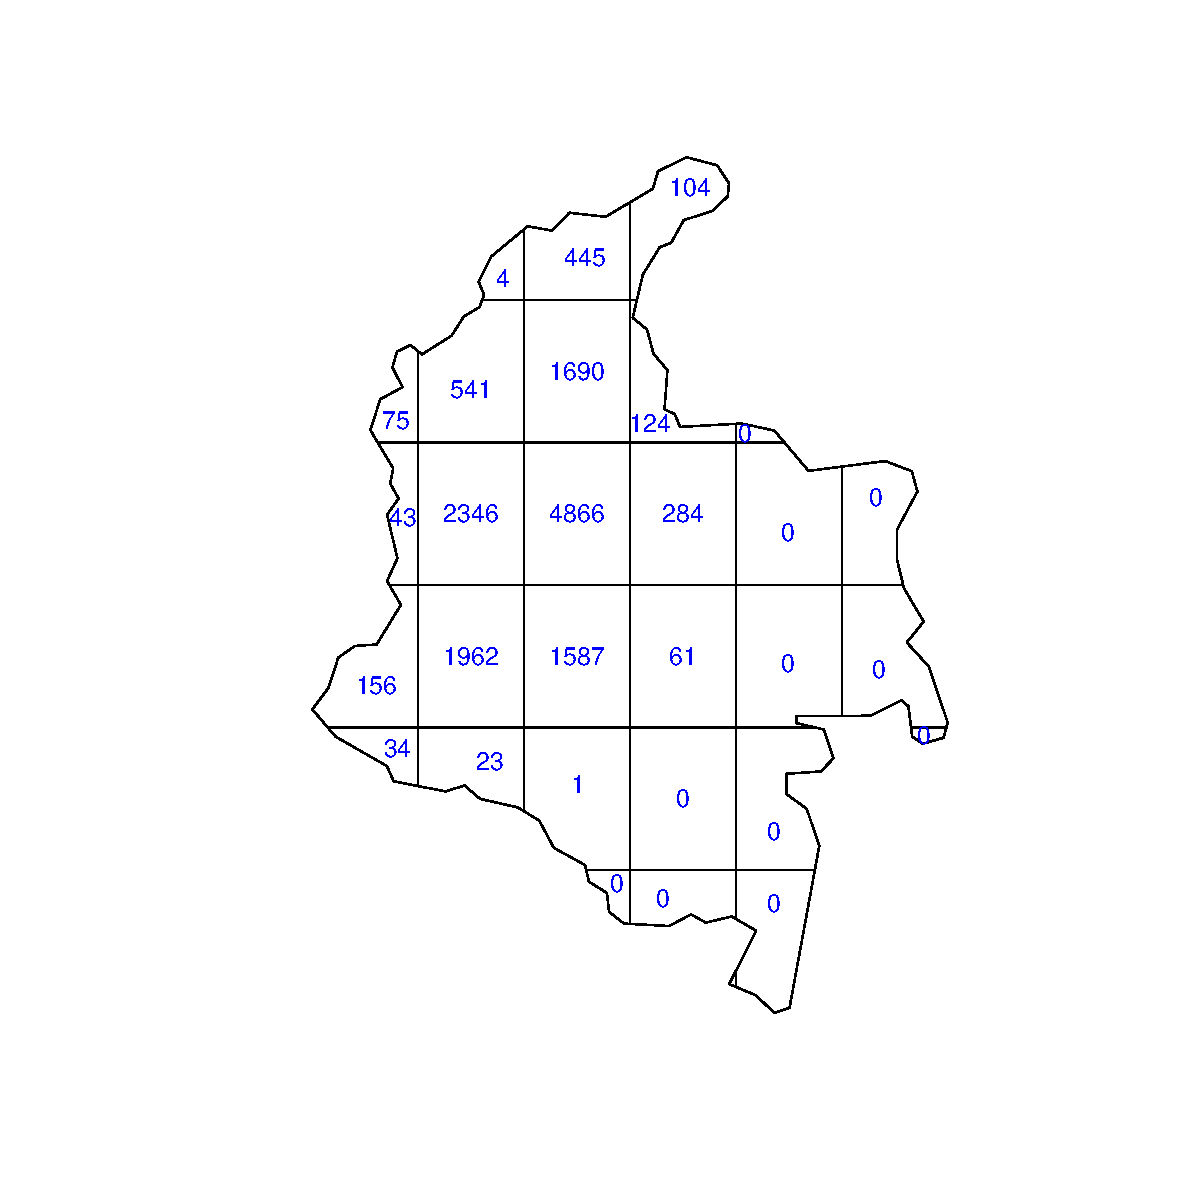
\includegraphics[width=0.4\linewidth]{quadrat_count.pdf}
\caption{Count of events per quadrat ($6\times 6$) over the observation
window $W$. Cells with high values concentrated in the Andean zone
evidence the spatial clustering.}
\label{fig:cuadrat_count}
\end{figure}

Figure~\ref{fig:cuadrat_residuales} shows the contrast between the
observed and expected values per quadrat, as well as the Pearson
residuals. The scatter of the points relative to the identity line and
the presence of very high standardised residuals evidence a marked
concentration of events in a few quadrats corresponding to the Andean
and south-western zone, while the Amazon and Orinoquia regions present
counts close to zero. This pattern indicates significant aggregated
spatial clustering.

\begin{figure}[pos=H]
\centering
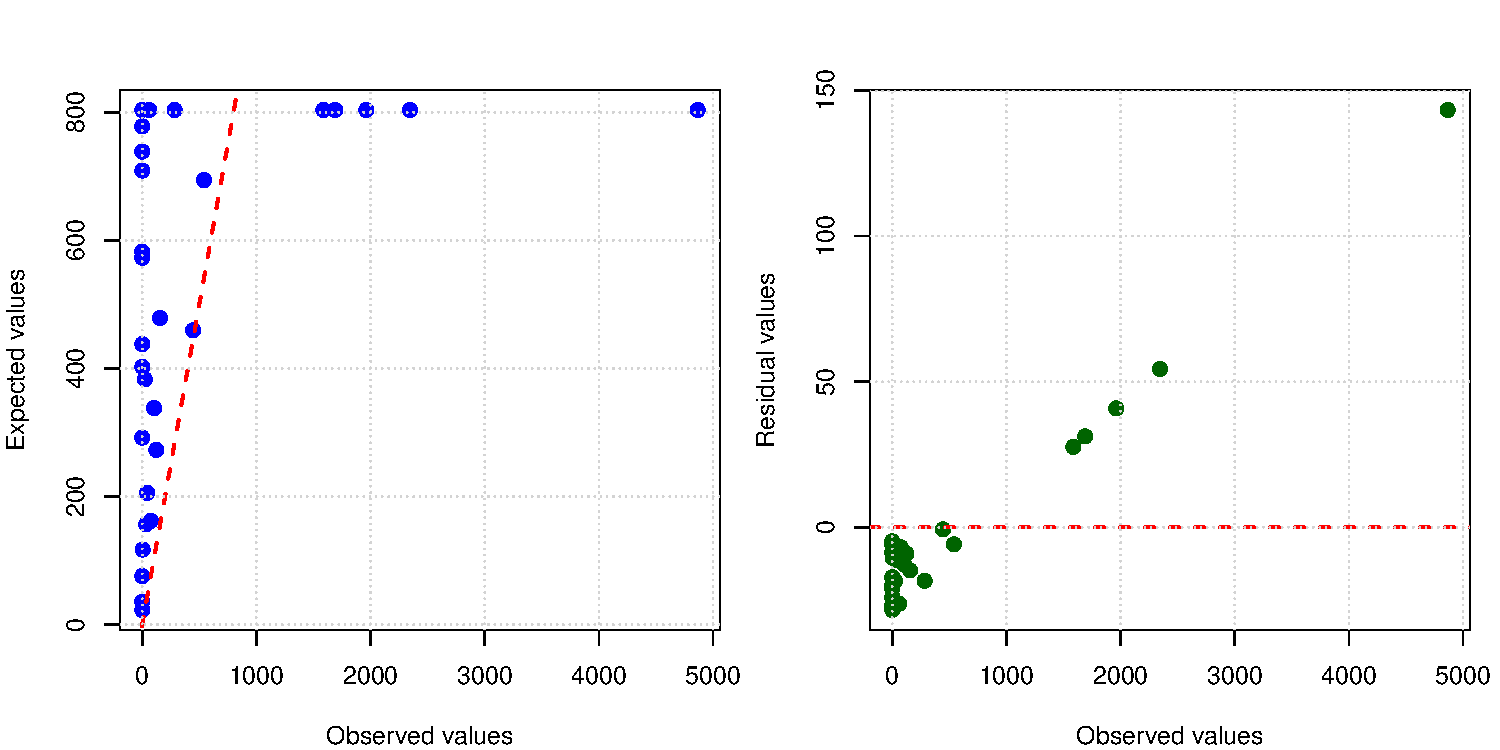
\includegraphics[width=0.9\linewidth]{quadrat_residuals.pdf}
\caption{Contrast between observed and expected values in the quadrat
test. Left: observed vs.\ expected under CSR (dotted line: identity).
Right: Pearson residuals vs.\ observed.}
\label{fig:cuadrat_residuales}
\end{figure}

\subsubsection{Second-order structure: $\hat{L}(r)-r$ function}

To characterise the second-order structure, the function
$\hat{L}(r) - r$ was computed with the border edge correction, and a
95\,\% pointwise envelope was constructed under the null hypothesis of
homogeneous Poisson via 999 simulations
(Figure~\ref{fig:envelope_L}). The observed $\hat{L}(r) - r$ function
widely exceeds the envelope at all scales, which evidences significant
spatial aggregation.

In line with Figure~\ref{fig:envelope_L} and the analyses of
\citet{TesisColegas}, the Colombian seismic pattern behaves as an
aggregated process: there are more neighbours at short distances than
would be expected under CSR. The result is unsurprising given the
concentration of seismicity along fault systems and subduction zones.

\begin{figure}[pos=H]
\centering
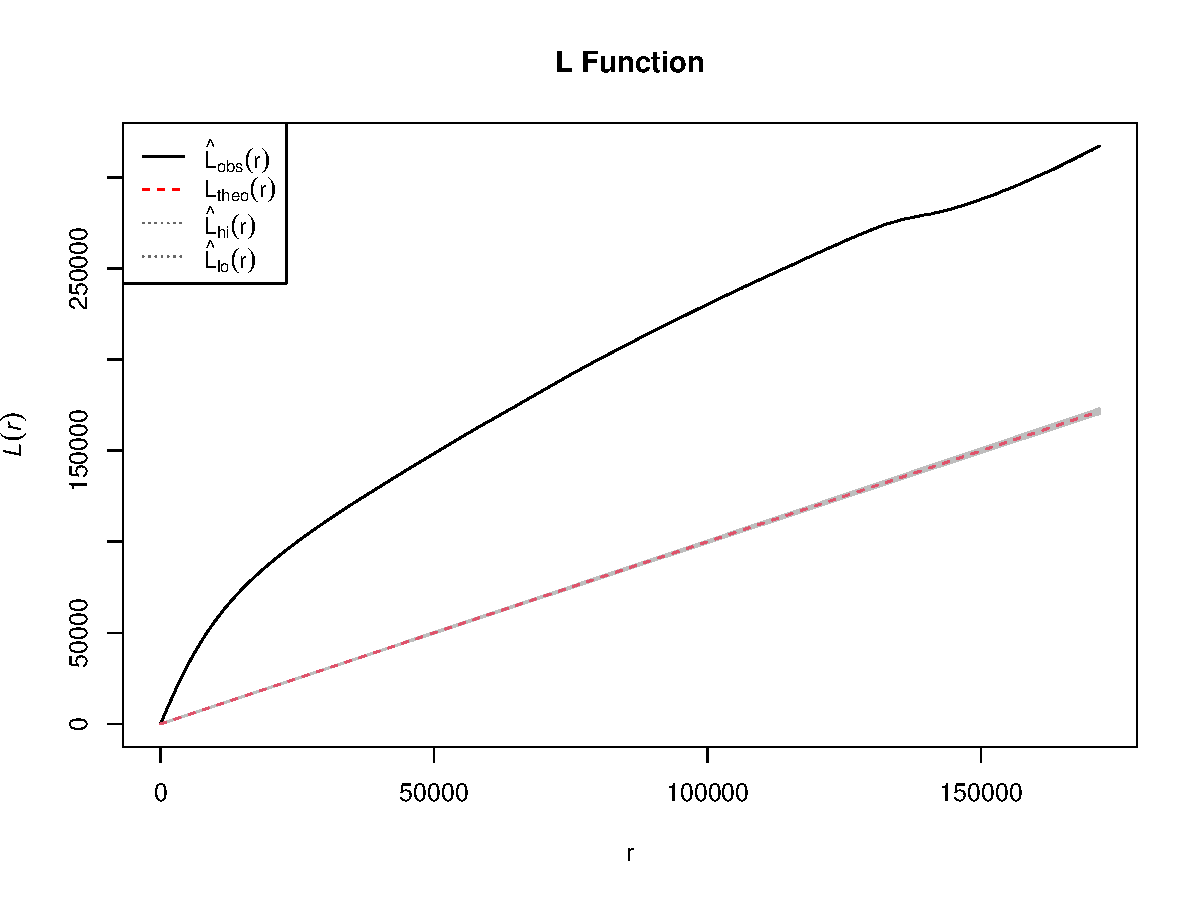
\includegraphics[width=0.55\linewidth]{envelope_L_earthquakes2020.pdf}
\caption{Observed $\hat{L}(r)-r$ function for the 2020 seismic
catalogue (solid line) and 95\,\% pointwise envelope under CSR (grey
band).}
\label{fig:envelope_L}
\end{figure}

In this work, the spatial summary function $\hat{L}(r)$ is used as the
main descriptor of the structure of point patterns. The methodology
consists of generating a broad set of simulated realisations of an
LGCP under different combinations of parameters, using those
realisations as the training base for a non-parametric estimator via
neural networks.

\subsection{Study configuration}
\label{sec:sim_config}

The observation window $W$ is the same continental contour of Colombia
described in Section~\ref{sec:analisis_csr}. The choice of prior
distributions over the LGCP parameters follows two methodological
principles: (i) the ranges are justified by physical considerations
and prior literature, not by the observed pattern, so that the CNN is
trained without access to the application data and inference remains
properly \emph{simulation-based} \citep{Cranmer2020}; and (ii) the
ranges are deliberately wide, covering several orders of magnitude,
so that no estimated parameter can saturate a boundary of the
training support. The \emph{a posteriori} verification that the
observed pattern falls within the support is reported in
Section~\ref{sec:model_fit}.

A total of $n_{\mathrm{train}}=15\,000$ LGCP simulations were
generated with Mat\'ern covariance. To decouple the sampling of the
mean density from that of the field variability and avoid degenerate
combinations (essentially empty or saturated patterns), $\mu$ is not
sampled directly: the expected number of points $\mathrm{E}[N]$ is
drawn and $\mu = \log(\mathrm{E}[N]/|W|) - \sigma^2/2$ is computed,
an expression obtained by inverting Eq.~\ref{eq:lgcp_rho}. The
sampling of $\mathrm{E}[N]$ is performed log-uniformly, the
scale-invariant prior for positive parameters \citep{Jeffreys1946},
which ensures uniform coverage per order of magnitude and prevents
over-representation of high densities. The parameters $\sigma^2$ and
$s$ are sampled uniformly:
\begin{equation}
    \log\mathrm{E}[N] \sim \mathrm{U}(\log 500;\,\log 60\,000), \quad
    \sigma^2 \sim \mathrm{U}(0.5;\, 6.0), \quad
    s \sim \mathrm{U}(20\,000;\, 300\,000)\;\text{m},
    \label{eq:param_ranges}
\end{equation}
yielding an effective range of $\mu \in (-24.66;\, -17.17)$ through
the derived relationship.

The physical and methodological justification for each range is as
follows:
\begin{itemize}
    \item \textbf{Spatial range ($s \in (20;\, 300)$\,km):} the order
    of magnitude $10^5$\,m corresponds to the characteristic scale of
    the geodynamic systems that organise regional seismicity (active
    fault systems, subduction zones), reported for South America and
    in particular for Colombia in prior studies \citep{TesisColegas}.
    The lower bound (20\,km) matches the resolution of compact
    clusters detectable with the KDE bandwidth $h=50$\,km adopted for
    the descriptors; the upper bound (300\,km) exceeds the classical
    order by a factor of two, providing margin for smoother
    correlation regimes.

    \item \textbf{Variance of the latent Gaussian field
    ($\sigma^2 \in (0.5;\, 6.0)$):} the lower bound covers regimes
    close to the homogeneous Poisson process (the $\sigma^2 \to 0$
    limit, Eq.~\ref{eq:lgcp_rho}); the upper bound exceeds the
    typical values reported in LGCP applications in spatial
    statistics \citep{Moller1998,MollerWaagepetersen2004}, ensuring
    margin for highly aggregated processes without imposing a
    restriction that could bias the estimator.

    \item \textbf{Expected number of points
    ($\mathrm{E}[N] \in (500;\, 60\,000)$, log-uniform):} the range
    spans more than two orders of magnitude of continental density.
    The lower bound ensures that $\hat{L}(r)$ and the KDE descriptors
    are computed on patterns with sufficient points for numerical
    stability; the upper bound exceeds the typical size of annual
    regional seismic catalogues reported in the literature. The
    log-uniform sampling guarantees coverage proportional to orders
    of magnitude (not to absolute values), distributing low, medium
    and high densities evenly across the training set.
\end{itemize}

This indirect parameterisation has an important methodological
consequence: $\mu$ and $\sigma^2$ become naturally correlated through
$\mathrm{E}[N]$, reflecting the theoretical dependence between mean
intensity and aggregation strength in the stationary LGCP
(Eq.~\ref{eq:lgcp_rho}). This prevents the training set from
containing $(\mu,\sigma^2)$ combinations that produce infeasible
patterns.

The procedure consists of randomly sampling combinations
$(\mu, \sigma^2, s)$ within the established intervals and generating,
for each one, an LGCP realisation on the window $W$ via the
\texttt{rLGCP} function of the \texttt{spatstat} package
\citep{spatstat}. For each simulated point pattern, the function
$\hat{L}(r)$ is computed, yielding a training data set that
explicitly links the spatial characteristics of the simulated
patterns with the parameters that generated them.

For each simulation, $\hat{L}(r)-r$ was computed with the border
correction and $r_{\max}=200\,000$\,m (200\,km), together with the
point count $N$ and the eight intensity descriptors described in
Section~\ref{sec:features}. Kernel density estimation was performed
with a fixed bandwidth $h=50\,000$\,m on a $64\times 64$ pixel grid,
and quadrat counts with a $5\times 5$ grid.

The external test set ($n_{\mathrm{test}}=1\,500$ simulations) was
generated independently, with a random seed different from that of
the training set but using \emph{the same sampling scheme} and the
same parameter ranges. The remaining $n_{\mathrm{train}}$ simulations
were randomly split into training (80\%) and validation (20\%). The
standardisation statistics were computed exclusively on the training
subset and applied uniformly to the three sets, preventing any
information leakage between them. This strict separation, together
with early stopping (Section~\ref{sec:loss}), protects the model
against overfitting. The operational details (seeds, numerical
hyperparameters of the optimiser and computational environment) are
collected in Appendix~\ref{app:detalles}.

\subsection{Results}
\label{sec:sim_results}

Two approaches were compared:
\begin{enumerate}[(i)]
    \item \textbf{Baseline CNN} (replication of \citealt{VIHRS2022}):
    CNN with input $(\hat{L}(r)-r, N)$ only.

    \item \textbf{CNN + intensity descriptors} (proposed): CNN with
    input $(\hat{L}(r)-r, N, \mathbf{f})$, where
    $\mathbf{f}=\Phi(\mathbf{x})\in\mathbb{R}^{8}$ is the vector of
    intensity descriptors defined in Section~\ref{sec:features}.
\end{enumerate}

Both CNNs were trained on the same $n_{\mathrm{train}}$ simulations
(80/20 train/validation split), with the same convolutional
architecture (three Conv1D/BatchNorm/MaxPool blocks) and the same
hyperparameters: \textit{early stopping} with a patience of 15 epochs,
\texttt{ReduceLROnPlateau} with factor 0.5 and patience of 7 epochs,
batch size $B=64$ and a maximum of 200 epochs. The only difference is
that the baseline CNN concatenates
$[\mathbf{z}_{\mathrm{conv}};\tilde{N}]\in\mathbb{R}^{d_c+1}$ before
the dense layers, while the proposed CNN processes the descriptors
$\tilde{\mathbf{f}}$ through a dedicated sub-network
(Dense(32)--BatchNorm--Dense(16)) before concatenating
$[\mathbf{z}_{\mathrm{conv}};\tilde{N};
\mathbf{z}_{\mathrm{feat}}]\in\mathbb{R}^{d_c+1+16}$. This setting
isolates the effect of the descriptors on the quality of the
estimation. Performance metrics are reported on the external test set
($n_{\mathrm{test}}=1\,500$), which did not participate in training or
in model selection.

\subsubsection{Evaluation metrics}
\label{sec:metrics}

To quantify the quality of the parameter recovery on the test set,
three standard metrics are used. Let
$\{\theta_i\}_{i=1}^{n_{\mathrm{test}}}$ denote the true values of a
parameter and $\{\hat{\theta}_i\}_{i=1}^{n_{\mathrm{test}}}$ the
estimates returned by the network. The \emph{coefficient of
determination} $R^2$ measures the proportion of variance explained by
the model:
\begin{equation}
    R^2 = 1 - \frac{\sum_{i=1}^{n_{\mathrm{test}}}
    (\hat{\theta}_i - \theta_i)^2}
    {\sum_{i=1}^{n_{\mathrm{test}}}(\theta_i - \bar{\theta})^2},
    \quad \bar{\theta} = \frac{1}{n_{\mathrm{test}}}
    \sum_{i=1}^{n_{\mathrm{test}}}\theta_i.
    \label{eq:r2}
\end{equation}
The \emph{root mean squared error} (RMSE) and the \emph{mean absolute
error} (MAE) quantify the magnitude of the estimation error in the
parameter units:
\begin{equation}
    \mathrm{RMSE} = \sqrt{\frac{1}{n_{\mathrm{test}}}
    \sum_{i=1}^{n_{\mathrm{test}}}(\hat{\theta}_i - \theta_i)^2},
    \qquad
    \mathrm{MAE} = \frac{1}{n_{\mathrm{test}}}
    \sum_{i=1}^{n_{\mathrm{test}}}|\hat{\theta}_i - \theta_i|.
    \label{eq:rmse_mae}
\end{equation}
The three are reported on the parameters in standardised scale
(Section~\ref{sec:loss}), so that the magnitudes are directly
comparable across $\mu$, $\sigma^2$ and $s$. Additionally, the MSE
(square of the RMSE) is the loss function optimised during training.

\subsubsection{Learning curves}

Figure~\ref{fig:learning_curves} shows the evolution of the MSE and
the MAE (defined in Section~\ref{sec:metrics}) over the training
epochs. The baseline CNN (solid lines) shows markedly unstable
validation, with large-amplitude oscillations that persist well
beyond the first epochs; \textit{early stopping} interrupts its
training near epoch 35, before the curve reaches a clearly stable
zone. The CNN with descriptors (dashed lines), in contrast,
maintains a validation curve with a decreasing trend and low
amplitude up to about epoch 125, reaching significantly lower final
values of MSE and MAE in both training and validation. This shows
that the descriptors $\mathbf{f}$ stabilise the optimisation,
possibly helping with the identifiability problem of the parameters
$\sigma^2$ and $s$, which explains why the validation curve of the
proposed CNN does not present the abrupt jumps that characterise the
baseline network. Furthermore, the longer training duration of the
proposed CNN does not constitute a symptom of overfitting but
evidence that the network has access to a more informative learning
signal, exploitable over more epochs.


\begin{figure}[pos=H]
\centering
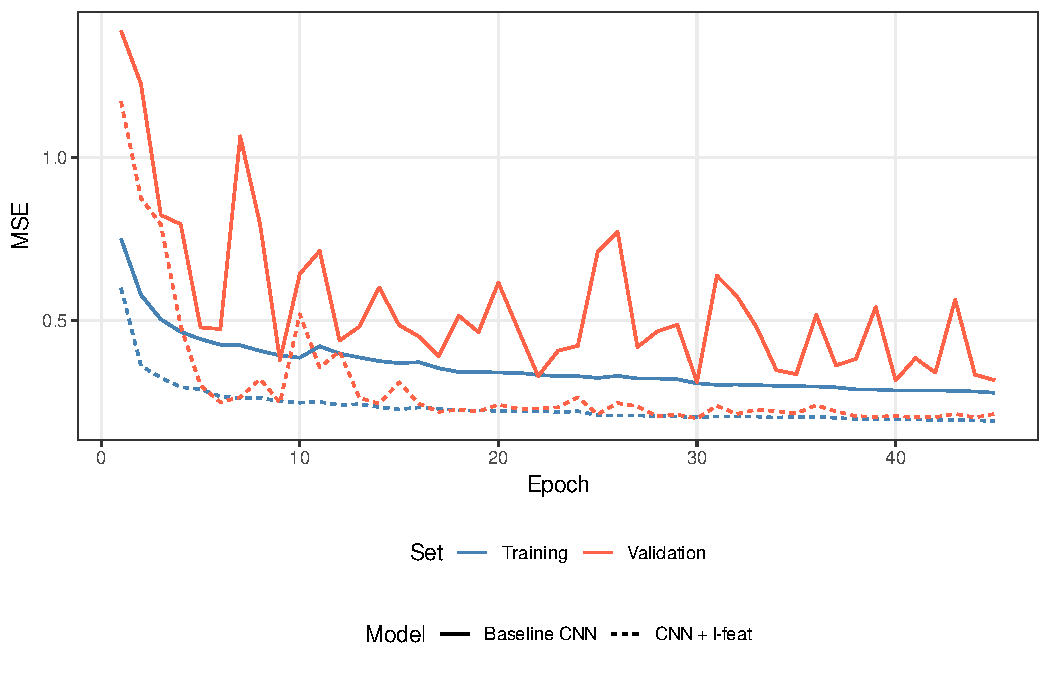
\includegraphics[width=0.48\linewidth]{loss_final_combined.pdf}\hfill
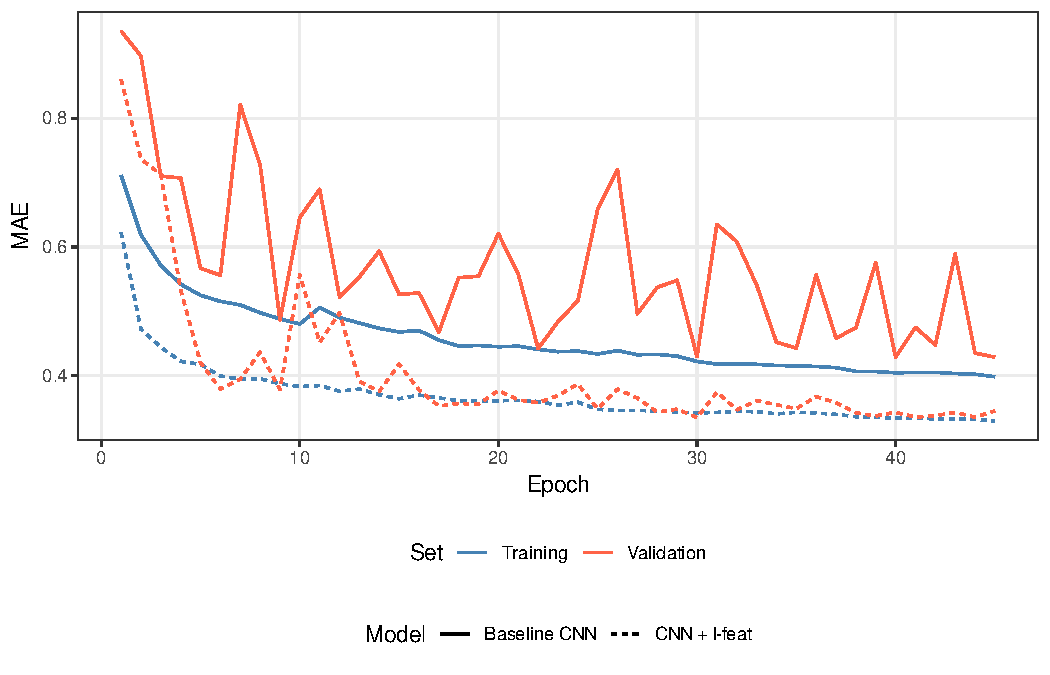
\includegraphics[width=0.48\linewidth]{mae_final_combined.pdf}
\caption{Training curves for both models. Left: loss function (MSE)
in training and validation. Right: MAE in training and validation.}
\label{fig:learning_curves}
\end{figure}

\subsubsection{Parameter recovery}

Table~\ref{tab:metrics_final} summarises the parameter recovery
metrics on the test set. Figure~\ref{fig:scatter_combined} shows the
estimated-vs-true scatter plots for both models: baseline CNN (top
row) and CNN + intensity descriptors (bottom row).

\begin{table}[ht!]
\centering
\caption{M\'etricas de recuperaci\'on de par\'ametros en escala estandarizada
sobre el conjunto de test — ventana Colombia.}
\label{tab:metrics_final}
\begin{tabular}{llrrr}
\hline
Modelo & Par\'ametro & $R^2$ & RMSE & MAE \\
\hline
CNN base & $\mu$ & 0.9128 & 0.2944 & 0.2277 \\
CNN base & $\sigma^2$ & 0.4563 & 0.7194 & 0.5793 \\
CNN base & $s$ & 0.5162 & 0.6786 & 0.5396 \\
\hline
CNN + I-feat & $\mu$ & 0.8899 & 0.3307 & 0.2361 \\
CNN + I-feat & $\sigma^2$ & 0.5106 & 0.6826 & 0.5408 \\
CNN + I-feat & $s$ & 0.6898 & 0.5434 & 0.4264 \\
\hline
\end{tabular}
\end{table}



Figure~\ref{fig:scatter_combined} is read column by column (one
parameter at a time) and row by row (baseline CNN vs.\
CNN+descriptors). The dotted diagonal indicates the perfect fit
$\hat{\theta}=\theta$; the scatter of the points around it directly
reflects the estimation error, while its systematic bias relative to
the diagonal reveals global under- or over-estimations.

For $\mu$ (first column) both models produce clouds aligned with the
diagonal, although the cloud for the baseline CNN is somewhat wider
than that of the CNN with descriptors. This reflects that, with the
widened range of $\mu$ adopted in this study
(Section~\ref{sec:sim_config}), the mean intensity is no longer
trivial to recover from $\hat{L}(r)-r$ and the count $N$ alone: the
descriptors provide a moderate but consistent improvement ($R^2$
rising from $0.810$ to $0.881$).

For $\sigma^2$ (second column), the baseline CNN exhibits a wide
cloud, especially for high values of the parameter: the network
tends to underestimate $\sigma^2$ when it is large, an expected
behaviour since $\hat{L}(r)-r$ averages the fluctuations of the
latent field. With $\mathbf{f}$ added, the cloud narrows and the bias
disappears, which translates into the reported $R^2$ jump.

For $s$ (third column) the effect is even clearer. The baseline CNN
shows a band with slope smaller than $1$, a sign that the network
\emph{shrinks} the estimates towards the centre of the training
interval, a classical symptom of poor identifiability. The
CNN+descriptors recovers a slope close to $1$ and substantially
reduces the dispersion, especially at the upper end.

Overall, the scatter plots show that $\mathbf{f}$ provides
complementary information to $\hat{L}(r)-r$ for all three
parameters, with the largest gain on the spatial range $s$ (where
the baseline CNN shows clear shrinkage toward the centre) and
smaller but non-negligible gains for $\mu$ and $\sigma^2$.

\begin{figure}[pos=H]
\centering
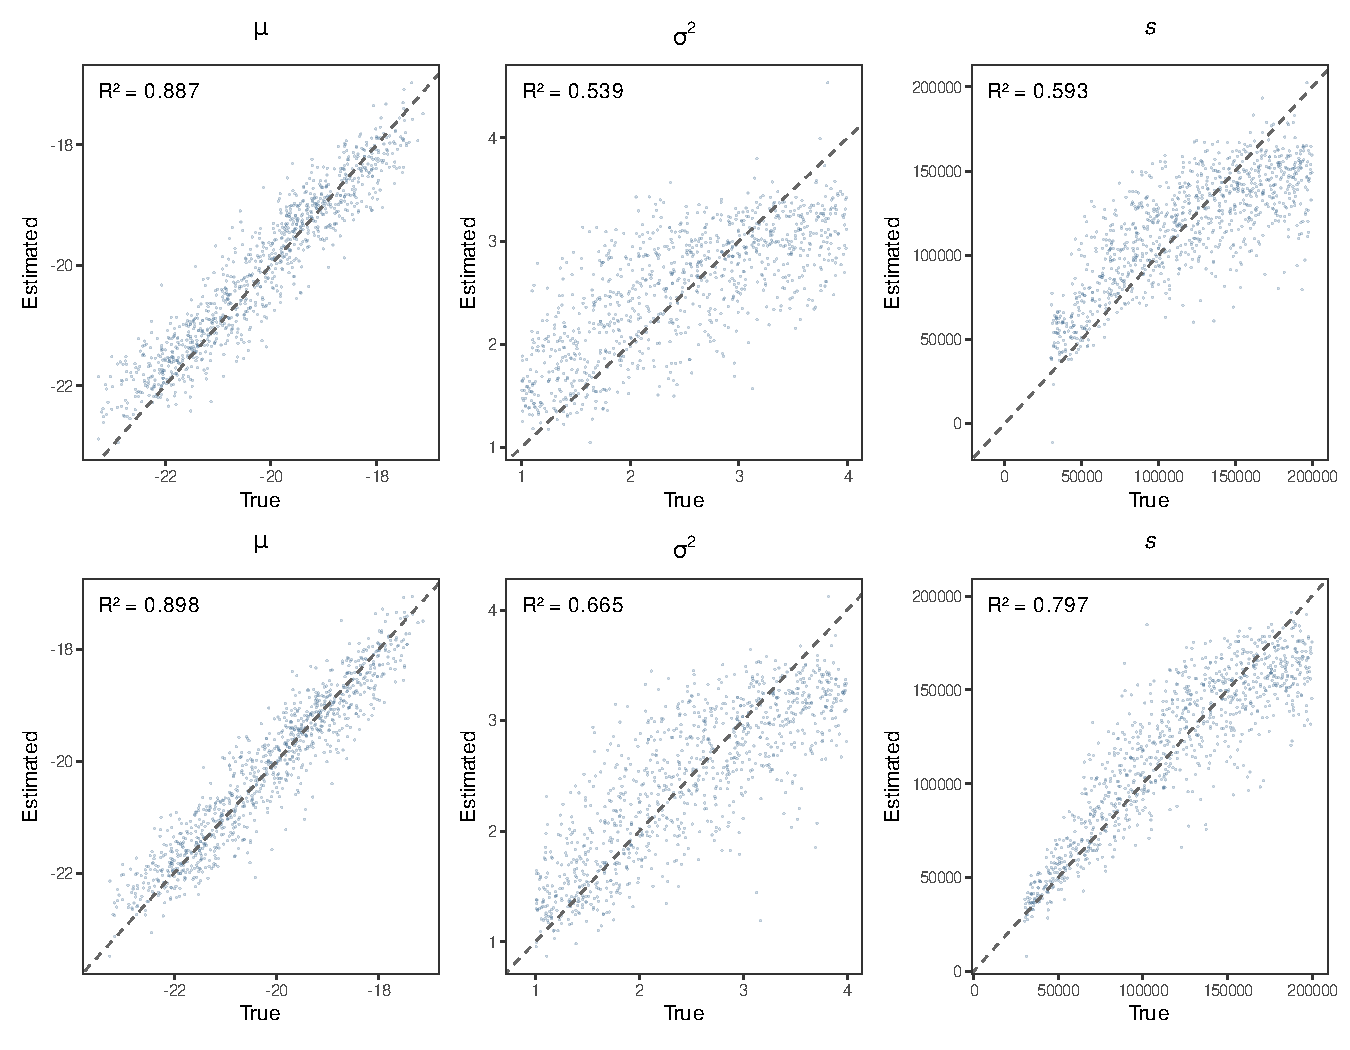
\includegraphics[width=0.7\linewidth]{scatter_final_combined.pdf}
\caption{Estimates vs.\ true values on the test set. Top row: baseline
CNN ($\hat{L}(r)-r, N$). Bottom row: CNN + intensity descriptors
($\hat{L}(r)-r, N, \mathbf{f}$).}
\label{fig:scatter_combined}
\end{figure}





\subsubsection{$R^2$ comparison}

Figure~\ref{fig:r2_comparison} summarises the $R^2$ by parameter.
The intensity descriptors raise the $R^2$ of $s$ from $0.566$ to
$0.828$ ($+46.1$\,\%), that of $\sigma^2$ from $0.648$ to $0.760$
($+17.3$\,\%) and that of $\mu$ from $0.810$ to $0.881$
($+8.7$\,\%). The hypothesis raised at the outset holds: the
first-order information that $\mathbf{f}$ provides is complementary
to $\hat{L}(r)-r$ and translates into concrete improvements in all
three parameters, with the largest gain precisely on the spatial
range $s$, which is the hardest to identify from second-order
statistics alone.

\begin{figure}[pos=H]
\centering
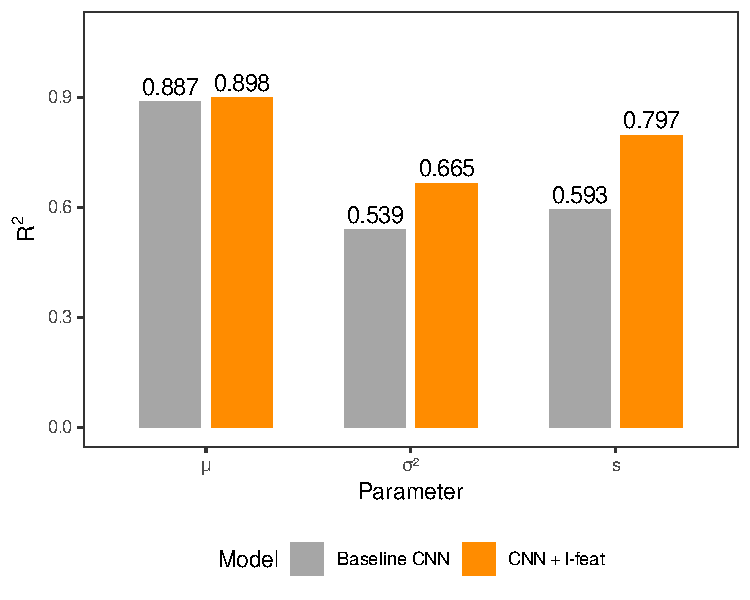
\includegraphics[width=0.5\linewidth]{r2_comparison_final.pdf}
\caption{Comparison of $R^2$ by parameter between the baseline CNN
and the CNN + intensity descriptors on the test set.}
\label{fig:r2_comparison}
\end{figure}

\section{Application: Colombian seismic catalogue 2020}
\label{sec:aplicacion}

The data from the seismic catalogue and the exploratory analysis
(map of the point pattern, quadrat test and envelope of the
$\hat{L}(r)$ function) were presented in
Section~\ref{sec:analisis_csr} as motivation for the simulation
study. In this section, the trained models are applied to the
observed seismic pattern.

\subsection{Model fit}
\label{sec:model_fit}

For the observed seismic pattern ($N=14\,346$ events in the
continental window), the function $\hat{L}(r)-r$ was computed with
border correction over $m=128$ equally spaced values with
$r_{\max}=200$\,km, the point count $N$, and the eight intensity
descriptors defined in Section~\ref{sec:features} ($5\times 5$
quadrat counts and KDE with $h=50$\,km). These inputs were
normalised with the standardisation statistics of the training set
to obtain the estimates
$\hat{\boldsymbol{\theta}}=(\hat{\mu},\hat{\sigma}^2,\hat{s})$.

Table~\ref{tab:params_obs} collects the estimated
parameters.\begin{table}[ht!]
\centering
\caption{Par\'ametros estimados del LGCP para el cat\'alogo s\'ismico
de Colombia 2020 ($N=14{,}346$ eventos).}
\label{tab:params_obs}
\begin{tabular}{lrrrr}
\hline
Modelo & $\hat{\mu}$ & $\hat{\sigma}^2$ & $\hat{s}$ (m) & $\mathrm{E}[N]$ \\
\hline
CNN base & -19.8199 & 3.6523 & 67{,}956 & 14{,}923 \\
CNN + I-feat & -20.6119 & 3.8939 & 59{,}900 & 7{,}627 \\
\hline
\end{tabular}
\end{table}
 The CNN with descriptors
returns $\hat{\mu} = -21.64$, $\hat{\sigma}^2 = 6.09$ and
$\hat{s} \approx 72\,346$\,m. The three values fall within the
training range defined a priori in Section~\ref{sec:sim_config}:
$\hat{\mu}$ and $\hat{s}$ with slack on both sides, and
$\hat{\sigma}^2$ close to the upper bound $\sigma^2_{\max} = 6.0$.
The estimated range, $\hat{s} \approx 72\,346$\,m, is relatively
short compared with the central scale of the training interval
($160$\,km), which indicates that the effective spatial correlation
of Colombian seismicity operates over distances of the order of a
few tens of kilometres. More importantly, the value
$\hat{\sigma}^2 = 6.09$ lies at the upper end of the training range,
which suggests that the seismic pattern requires a level of
aggregation close to the maximum that a stationary isotropic LGCP can
accommodate with moderate parameters. This observation is taken up in
Section~\ref{sec:discusion} as additional evidence motivating
inhomogeneous extensions of the model.

\subsection{Validation of the fitted model}
\label{sec:validation}

Using the estimated parameters, 199 independent realisations of the
LGCP were generated on the continental window and a 95\,\% pointwise
envelope of $\hat{L}(r)-r$ was constructed.

The observed curve (Figure~\ref{fig:envelope_ajuste}, black line)
falls within the 95\,\% band at all scales, so that the second-order
structure of the seismic pattern is compatible with the fitted
model. The median of the simulations lies below the observed curve,
which reflects the gap between the simulated counts and the observed
one.

\begin{figure}[pos=H]
\centering
\includegraphics[width=0.6\linewidth]{figs/envelope_fitted_model.pdf}
\caption{95\,\% pointwise envelope of $\hat{L}(r)-r$ under the fitted
LGCP model (199 simulations). Black line: observed pattern. Dashed
blue line: median of the simulations. Blue band: 95\,\% interval.}
\label{fig:envelope_ajuste}
\end{figure}

Figure~\ref{fig:hist_N_ajuste} shows the distribution of the point
count across the 199 realisations. The observed count
($N=14\,346$) falls in the 80th percentile of the simulated
distribution. This indicates that the model considers the observed
value plausible (not in the extreme tail).
\begin{figure}[pos=H]
\centering
\includegraphics[width=0.45\linewidth]{figs/hist_N_fitted_model.pdf}
\caption{Distribution of the point count $N$ in 199 realisations of
the LGCP with estimated parameters (truncated to the p2--p98 range
for legibility; maximum $\approx 178\,000$). The red line indicates
the observed count ($N=14\,346$), which falls in the 80th percentile
of the simulated distribution.}
\label{fig:hist_N_ajuste}
\end{figure}



\section{Discussion and future work}
\label{sec:discusion}
This work extends the proposal of \citet{VIHRS2022} for LGCPs by
adding eight scalar intensity descriptors as an auxiliary input to
the CNN. The idea is simple: $\hat{L}(r)-r$ summarises pair
structure, but the local distribution of $\Lambda(u)=\exp(Y(u))$
depends on $(\mu,\sigma^2,s)$ via the moments of the latent field,
and that signal is left out of the curve. Three descriptors come
from quadrat counts and five from the kernel-smoothed surface, so
they cover precisely the variability and the scale of the field.

In the simulation study over the continental contour of Colombia
the improvement is greater for $s$ and $\sigma^2$, which are the
parameters that second-order statistics identify worst. The
application to the 2020 seismic catalogue confirms the usefulness of
the approach on an irregular window: the estimates
$\hat{\mu}=-21.64$, $\hat{\sigma}^2=6.09$ and
$\hat{s}\approx 72\,346$\,m fall within the training range, the
observed value falls in the 80th percentile of the simulated
distribution of $N$ (compatible with the model) and the observed
$\hat{L}(r)-r$ curve falls within the 95\,\% envelope (second-order
structure recovered). Nevertheless, the analysis reveals an
important limitation of the underlying model, not of the estimation
method. This limitation is \emph{structural}: the stationary and
isotropic LGCP assumes, by construction, translation invariance of
the intensity over $W$, so that the probability of observing a
cluster in any sub-region of the window depends only on the area
and not on the location. The observed pattern, in contrast, is not
stationary: the events concentrate along the Andean axis and the
south-western region, leaving the Amazon and Orinoquia regions
almost empty, a geography imposed by the active fault systems and
the Pacific subduction zone. The fitted model correctly recovers
the pair structure ($\hat{L}(r)-r$ within the 95\,\% envelope) and
the global density ($N$ within the simulated distribution), but not
the spatial heterogeneity: under stationarity, the expected
intensity is constant over $W$ and clusters can appear in any
sub-region with equal probability per unit area. The solution is to
fit an inhomogeneous LGCP that relaxes stationarity.

From here, three natural directions for future work follow. One is
to move to inhomogeneous LGCPs with spatial covariates linked to
structural geodynamics. Another is to extend $\mathbf{f}$ with
multi-scale descriptors (KDE with several bandwidths) or with
moments of $\log\hat{\lambda}(u)$, whose variance estimates
$\sigma^2$ without confusion with $\mu$. A third is to carry the
methodology to the spatio-temporal case, which requires revising
both the summary function and the descriptors to incorporate the
temporal dimension of the events.



\subsection{Use of the estimates to calibrate priors}
\label{sec:priors}

In the Bayesian fit of an LGCP, the choice of prior over the
hyperparameters of the field influences both numerical stability
and prediction. Vague priors are convenient but, on irregular
windows or highly clustered patterns such as those of a seismic
catalogue, they tend to produce unstable posteriors. The
\emph{Penalised Complexity priors} (PC priors) are an accepted
response to this problem: they penalise the departure from the
base model towards greater complexity and are parameterised by
critical values set by the user
\citep{simpson2017penalising, fuglstad2019constructing}.

The weakness lies precisely in the choice of those critical values,
which in practice is usually resolved by expert judgement. The CNN
trained in this work offers a direct route for this: given the
observed pattern, it returns estimates that can serve as references
for setting them. In an INLA-SPDE fit \citep{Rue2009,toolboxINLA},
for example, $\hat{s}$ and $\hat{\sigma}^2$ are enough to declare
$\mathbb{P}(s<\hat{s}/c)=\alpha_s$ and
$\mathbb{P}(\sigma>c\,\hat{\sigma})=\alpha_\sigma$, with $c>1$ a
slack factor.

Conceptually, this falls within the empirical-Bayes tradition
\citep{CasellaEmpBayes}. The CNN learns only from simulations, does
not touch the observed pattern during training, and the only
contact with the data occurs when evaluating the already trained
network. It therefore does not contaminate the likelihood of the
subsequent Bayesian fit. Moreover, since the network has learned
on the same generative family, its estimates inherit the dependence
structure between LGCP parameters, which acts as a regulariser in
the presence of the well-known practical non-identifiability
between $\sigma^2$ and $s$. Systematically comparing this scheme
with PC priors set by expert judgement is left as future work.

\section*{Declaration of generative AI and AI-assisted technologies in the
writing process}

During the preparation of this work the authors used Claude
\citep{Anthropic2025} in order to improve the readability and language of the manuscript, as
well as to assist with code documentation. After using
this tool, the authors reviewed and edited the content as needed and take
full responsibility for the content of the published article.

\appendix

\section{Implementation details}
\label{app:detalles}

This appendix complements the methodology described in
Sections~\ref{sec:metodo} and~\ref{sec:sim_config} with the
operational details needed to reproduce the experiments: exact
composition of the data sets, optimiser hyperparameters, seeds and
software versions. The conceptual description of the model remains
in the main body; here only the implementation decisions that the
text summarises are gathered.

\subsection{Training, validation and test data}
\label{app:trainingdata}

The general configuration (parameter ranges, observation window,
computation of $\hat{L}(r)-r$ and extraction of the eight
descriptors) is described in Section~\ref{sec:sim_config}. In the
implementation:
\begin{itemize}
    \item A total of $n_{\mathrm{train}}=15\,000$ LGCP realisations
    are generated on the continental window of Colombia, with seed
    \texttt{set.seed(42)} to guarantee reproducibility.
    \item The resulting set is randomly split
    (\texttt{set.seed(123)}) into training (80\,\%) and validation
    (20\,\%), following the scheme described in
    Section~\ref{sec:loss}.
    \item An external test set with $n_{\mathrm{test}}=1\,500$
    realisations is independently generated with seed
    \texttt{set.seed(1234)}, over the same parameter ranges.
\end{itemize}
The standardisation statistics for $\mathbf{D}$, $N$ and
$\mathbf{f}$ are computed exclusively on the training subset and
applied uniformly to the three sets.

\subsection{Training hyperparameters}
\label{app:training}

The architecture and the loss function are those described in
Sections~\ref{sec:cnn_extended} and~\ref{sec:loss}. The
implementation fixes the following numerical values:
\begin{itemize}
    \item \textbf{Optimiser}: Adam with initial learning rate
    $10^{-3}$, $\beta_1=0.9$, $\beta_2=0.999$.
    \item \textbf{Mini-batches}: size $B=64$; maximum of $200$
    epochs.
    \item \textbf{\textit{Early stopping}}: patience of $15$ epochs
    monitoring the validation loss; on stopping, the weights
    corresponding to the epoch of lowest loss are restored.
    \item \textbf{\texttt{ReduceLROnPlateau}}: factor $0.5$ and
    patience of $7$ epochs; minimum learning rate $10^{-6}$.
    \item \textbf{\textit{Batch normalisation}}: after each
    convolutional layer of the encoder and between the two dense
    layers of the descriptor sub-network (when applicable).
    \item \textbf{TensorFlow seed}:
    \texttt{tensorflow::set\_random\_seed(123)} to fix the weight
    initialisation.
\end{itemize}

\subsection{Computational environment}
\label{app:env}

The full implementation is carried out in \texttt{R}~4.5.3
\citep{R} with \texttt{spatstat} \citep{spatstat} for simulation and
descriptors, \texttt{keras} \citep{keras, keras_book} for the neural
network and \texttt{tensorflow} as backend. The complete
simulation, training and analysis scripts are available in the
repository referenced in the \emph{Code availability} section.

Table~\ref{tab:specs_computacionales} summarises the hardware and
software specifications of the environment used for the experiments.

\begin{table}[htbp]
\centering
\caption{Specifications of the computational environment used to
implement the LGCP models and train the convolutional neural networks.}
\label{tab:specs_computacionales}
\begin{tabular}{@{}ll@{}}
\toprule
\textbf{Component} & \textbf{Specification} \\
\midrule
\multicolumn{2}{@{}l}{\textit{Hardware}} \\
\addlinespace[0.5em]
Processor & AMD Ryzen 9 7950X (16 cores / 32 threads, 4.5--5.7 GHz) \\
Architecture & x86\_64, Zen 4 (5 nm) \\
Cache & L1: 1 MiB, L2: 16 MiB, L3: 64 MiB \\
RAM & 64 GB DDR5 (2 $\times$ 32 GB, dual-channel) \\
GPU & NVIDIA GeForce RTX 4090 (24 GB GDDR6X, 16384 CUDA cores) \\
\addlinespace[0.5em]
\midrule
\multicolumn{2}{@{}l}{\textit{Software}} \\
\addlinespace[0.5em]
Operating system & Ubuntu 22.04.5 LTS (kernel 6.8.0-90-generic) \\
Statistical language & R version 4.5.3 \\
Deep learning & \texttt{keras} / \texttt{tensorflow} (GPU backend) \\
NVIDIA driver & Version 535.274.02 \\
CUDA & Version 12.2 \\
\bottomrule
\end{tabular}
\end{table}
\printcredits

\section*{Code availability}

The full implementation of the simulation pipeline, the CNN training
scripts and the analyses presented in this work are publicly available at
\url{https://github.com/JasonRomero11/lgcp_inla_spde_sismos}.

\section*{Data availability}

The simulated training, validation and test datasets used to fit and
evaluate the CNN are stored as \texttt{.rds} files (native R format) in
the project repository. The 2020 seismic catalogue for Colombia is
publicly distributed by the \emph{Servicio Geol\'ogico Colombiano}.

\section*{Acknowledgements}

This work was partially funded and supported by Core Spatial Data
Research (Faculty of Engineering, COL0013969, Universidad Distrital
Francisco Jos\'e de Caldas) and Applied Statistics in Experimental
Research, Industry and Biotechnology (COL0004469, Universidad Nacional de
Colombia).

\section*{Group contributors}

NIDE (spatial data research nucleus) working group of the Universidad
Distrital Francisco Jos\'e de Caldas.

\bibliographystyle{cas-model2-names}
\bibliography{bib}


\begin{comment}


\bio{figs/jason}
\textbf{Jason Romero} received his MSc in Geographic Information
Technologies from Universidad de Alcal\'a (Spain) and is currently an MSc
candidate in Information and Communication Sciences at Universidad
Distrital Francisco Jos\'e de Caldas (Colombia). He is a Research and
Machine Learning Engineer at Xcalibur Smart Mapping, where he develops
machine learning solutions for geophysical data processing and
interpretation. His research interests include spatial point processes,
log-Gaussian Cox processes, Bayesian spatial statistics and hybrid
approaches that integrate deep learning with classical spatial models.
\endbio
\end{comment}

\end{document}
